% Um alles auf einmal pflegen zu können, verwenden wir \ifhtml als
% Anzeige für tex4ht oder „normales“ (PDF)LaTeX.
%
\makeatletter

\let\ifhelp\iffalse
\let\ifhtml\iffalse
\let\ifpdf\iffalse
\let\ifdvi\iffalse

\def\mutabor@utput@html{
  \typeout{Producing HTML format.}
  \let\ifhtml\iftrue
}

\def\mutabor@utput@help{%
  \mutabor@utput@html
  \typeout{Subtype: .hhp .}
  \let\ifhelp\iftrue
}

\@ifundefined{mutabor@utput@\outputformat}{
  \typeout{Undefined output format%
    \@ifundefined{outputformat}{}{ \outputformat}.
  }
}{
  \csname mutabor@utput@\outputformat\endcsname
}

%\def\htmltrue{\let\ifhtml\iftrue}
%\def\htmlfalse{\let\ifhtml\iffalse}
%\ifx\ifhtml\undefined
%  \htmlfalse
%\else
%  \htmltrue
%\fi
% 
% Ein Kommentar aus dem alten Handbuch... ;-)
%
% =====================================================
%
% NOCH ZU KORRIGIEREN :
%
%
% - oberflächenspezifische Beschreibungen auslagern !
%
% =====================================================
%
% Koma-Skript liefert ein paar nützliche zusätzliche Definitionen
%
\documentclass[german,a4paper,BCOR1.0cm]{scrbook}
%
% Für tex4ht müssen wir auch tex4ht laden...
\ifhtml
\setcounter{tocdepth}{1}
% Grundeinstellungen liegen in der Datei „tshtml.cfg“
\usepackage[%tshtml,
mutabor,
% Es folgt das Hauptformat: hier xhtml
            html,
% CSS2 verwenden
%            css2,
% in der Log-Datei Informationen zur Konfiguration von tex4ht ausgeben
          info,
% Fußnoten (und Literaturzitate) erscheinen beim überfahren der Marke
%            mouseover,
% Auf der ersten Seite wird auch ein „Weiter“-Pfeil angezeigt
            next,
            sections+,
% HTML-Dateien möglichst kurz -- maximale Aufsplittungstiefe
            4,
 %            nominitoc,
% Index 2-Spaltig
            index=2,
            Gin-dim+,
% HTML-Zeichensatz: UTF-8
            charset=utf-8,
            hyperref,
            NoFonts,
%            fonts+
%            fonts,
]{tex4ht}
\makeatletter
\edef\ts@savecatcode{\noexpand\catcode`\noexpand\:\the\catcode`\:\relax} 
%\catcode`\:11\relax
\AtEndDocument{\makehhk}
\newcommand\tshhkentry{}
\newcommand\tsatoclink{}

%\:::HRefTag=macro:
%#1#2->\if \relax #2\relax \else \:TagHTag {#2}\fi \HCode {<\tag:A \:newlnch \if
% \relax #1\relax \NOHREF: {#2}\else \HREF: "\get:hfile {#1}\:sharp #1"\fi \if \
%relax #2\relax \else \space \NAME: "#2"\fi \:attr \empty:lnk >}.
%<insert>    \show\:::HRefTag

\expandafter\def\expandafter\mut@sharp\expandafter{\csname :sharp\endcsname}

\newif\ifwx@inrange
\wx@inrangefalse
\def\wx@item#1{%
  \def\wx@item@{#1}%
  \let\wx@indextext\wx@item@
}
\def\wx@subitem#1{%
  \def\wx@subitem@{\wx@item@{}: #1}
  \let\wx@indextext\wx@subitem@
}
\def\wx@subsubitem#1{%
  \def\wx@subsubitem@{\wx@subitem@{} -- #1}%
  \let\wx@indextext\wx@subsubitem@
}
\def\wx@LNK#1#2#3#4{%
  \ifwx@inrange
  \wx@inrangefalse
  \else
  \HCode{<li>^^J}%
  \HCode{<object type="text/sitemap" >^^J%
\space<param name="Name" value="}\wx@indextext\HCode{" >^^J%
\space<param name="Local" value="}#1\mut@sharp #2\HCode{" >^^J%
</object>^^J}% 
  \HCode{</li>^^J}%
  \fi
}
\def\loadwxindex{%
  {%
    \let\item\wx@item
    \let\subitem\wx@subitem
    \let\subsubitem\wx@subsubitem
    \let\LNK\wx@LNK
    \let\rangeto\wx@inrangetrue
    \InputIfFileExists{\jobname.wxi}{}{}%
  }%
}



\def\tsatoclink#1#2#3#4{%
  \typeout{Setting: \csname get:hfile\endcsname{#2} at \csname :sharp\endcsname #2}%
  \HCode{%
\tslinestart<object type="text/sitemap" >^^J
\tslinestart\space<param name="Name" value="}#4\HCode{" >^^J
\tslinestart\space<param name="Local" value="}\csname get:hfile\endcsname{#2}\csname :sharp\endcsname #2\HCode{" >^^J
\tslinestart</object>^^J}% "<
%   \expandafter\ifx \csname #3-def\endcsname\relax
%      \global \expandafter\let \csname #3-def\endcsname\def
%      \Link {#2}{#3}
%   \else
%      \Link {#2}{}
%   \fi 
%   {\Configure {ref}{}{}{}%
%     \let \EndLink =\empty
%     \let \H:Tag:attr \:gobbleII
%     \let \:::HRef \empty
%     \def \::hRef [##1]##2{}%
%     \def \::hRefTag [##1]##2##3{}%
%     \def \:::HRefTag ##1##2{}%
%     \Configure {cite}{}{}{}{}%
%     #4}%
%   \EndLink
}
\def\ts@hhkentry#1#2#3#4{%
  \def\tslinestart{#1\space}%
  \HCode{#1<li>^^J}%
  #3%
  \HCode{#1</li>^^J}%
}
\def\tshhkentry{\ts@hhkentry{}}
\def\tstocendsubparagraph{}
\def\tstocendparagraph{\endsubparagraph}

\def\deftocmacro#1#2#3{
  \expandafter\def\csname tstocstart#1\endcsname{%
    \HCode{#3\space<ul><!-- u#1 -->^^J}%
    \expandafter\let\csname tocstart#1\endcsname\relax
    \expandafter\def\csname tocstop#1\expandafter\endcsname{\csname tstocstop#1\endcsname}
  }

  \expandafter\def\csname tstocskip#1\endcsname{\csname tocstop#2\endcsname}

  \expandafter\def\csname tstocstop#1\endcsname{%
    \csname tocstop#2\endcsname
    \HCode{#3\space</ul><!-- i#1 -->^^J}%
    \expandafter\def\csname tocstop#1\endcsname{\csname tstocskip#1\endcsname}
  }

  \expandafter\def\csname tstoc#2\endcsname{%
    \csname tocstop#2\endcsname
    \csname tocstart#1\endcsname
    \expandafter\def\csname tocstart#2\endcsname{\csname tstocstart#2\endcsname}
    \HCode{#3\space\space<!-- a#2 -->^^J}%
    \ts@hhkentry{#3\space\space}%
  }%
}

\def\tstocpart{
  \tocstoppart
  \ts@hhkentry{}%
}

\deftocmacro{part}{chapter}{}
\deftocmacro{chapter}{section}{\space}
\deftocmacro{section}{subsection}{\space\space}
\deftocmacro{subsection}{subsubsection}{\space\space\space}
\deftocmacro{subsubsection}{paragraph}{\space\space\space\space}
\deftocmacro{paragraph}{subparagraph}{\space\space\space\space\space}
\def\tocstopsubparagraph{}

\def\gobblenl{\@ifnextchar[\@gobblenl{}}
\def\@gobblenl[#1]{}
{\catcode`\^^J=\active
  \gdef\mknlsp{%
    \def^^J{ }}%
}
\def\@nl@end{nl@end}
\def\@removenl#1#2\@nl@end{%
  \ifx#1^^J
  \ 
  \else
  #1
  \fi
  \ifx#2\relax
  \else
  \expandafter\@removenl
  \fi
}

\newcommand\removenewline[1]{%
  \ifx#1\relax
  \else
    \@removenl#1\@nl@end
  \fi
}

\newcommand\mutabortitle{}
\ifhelp
  \let\mutaborsavesubject\subject
  \def\subject#1{%
    \def\mutabortitle{#1}%
    \mutaborsavesubject{#1}%
  }
\else
  \let\mutaborsavetitle\title
  \def\title#1{%
    \def\mutabortitle{#1}%
    \mutaborsavetitle{#1}%
  }
\fi
\def\mutabordefaulttopic{\jobname.html}
\newcommand\tsarg{}
\def\tsarg#1{#1}
\let\tsdotocentry\tsarg
\expandafter\let\expandafter\mut@gobbleIV\csname :gobbleIV\endcsname
\expandafter\let\expandafter\mut@gobbleIII\csname :gobbleIII\endcsname
\expandafter\let\expandafter\mut@gobble\csname :gobble\endcsname
\newcommand\makehhk{%
  {\ignorespaces
    \let\par\relax
    \def\showname##1{\expandafter\show\csname ##1\endcsname}%
    \let\@gnewline\space
    \def\@newline{\space\mut@gobbleIII}%
    \let\texorpdfstring\@secondoftwo%
    \let\fontencoding\mut@gobble
    \let\fontfamily\mut@gobble
    \let\fontseries\mut@gobble
    \let\fontshape\mut@gobble
    \let\fontsize\mut@gobble
    \let\@setfontsize\mut@gobbleIII
    \let\usefont\mut@gobbleIV 
    \let\selectfont\relax
    \let\LARGE\relax
    \let\normalsize\relax
    % .hhp-Datei erstellen.
    \special{t4ht>\jobname.hhp}%
    \HCode{%
Contents file=\jobname.hhc^^J%
Index file=\jobname.hhk^^J%
Title=}{%
      \removenewline\expandafter{\mutabortitle}}%
    \HCode{^^J%
Default Topic=\mutabordefaulttopic^^J
Charset=UTF-8^^J}%
\special{t4ht<\jobname.hhp}%
\typeout{done}%
%\expandafter\show\csname a:TocLink\endcsname
    \let\doTocEntry\tsdotocentry
    \expandafter\let\csname a:TocLink\endcsname\tsatoclink
    \let\toclikesection\tshhkentry
    \let\toclikechapter\tshhkentry
    \let\tocaddchap\tshhkentry
    \let\tocpart\tshhkentry
    \let\tocsection\tshhkentry
    \let\tocchapter\tshhkentry
    \let\tocsubsection\tshhkentry
    \let\tocparagraph\tshhkentry
    \let\tocappendix\tshhkentry
    \let\tocminisec\tshhkentry
    \let\textsc\tsarg%
    \special{t4ht>\jobname.hhk}%
    \HCode{<ul>^^J}%
    \loadwxindex 
%    \catcode`\#11
    \InputIfFileExists{\jobname.4ct}{}{}%
\typeout{finished}%
    \HCode{</ul>^^J}%
    \special{t4ht<\jobname.hhk}%
\typeout{closed}%
%
    \let\toclikesection\tstocsection
    \let\toclikechapter\tstocchapter
    \let\tocaddchap\tstocchapter
    \let\tocpart\tstocpart
    \let\tocsection\tstocsection
    \let\tocchapter\tstocchapter
    \let\tocsubsection\tstocsubsection
    \let\tocparagraph\tstocparagraph
    \let\tocappendix\tstocchapter
    \def\tocminisec{\tocparagraph}%
%
    \let\tocstartpart\relax
    \let\tocstoppart\tstocskippart
    \let\tocstartchapter\relax
    \let\tocstopchapter\tstocskipchapter
    \let\tocstartsection\relax
    \let\tocstopsection\tstocskipsection
    \let\tocstartsubsection\relax
    \let\tocstopsubsection\tstocskipsubsection
    \let\tocstartsubsubsection\relax
    \let\tocstopsubsubsection\tstocskipsubsubsection
    \let\tocstartparagraph\relax
    \let\tocstopparagraph\tstocskipparagraph
    \let\tocstartsubparagraph\relax
    \let\tocstopsubparagraph\tstocskipsubparagraph
%
    \special{t4ht>\jobname.hhc}%
    \HCode{<ul>^^J}%
%    \catcode`\#11
    \InputIfFileExists{\jobname.4ct}{}{}%
    \HCode{</ul>^^J}%
    \special{t4ht<\jobname.hhc}%
  }%
  \relax
}
\fi
% Einstellungen für Latex laden
\usepackage[utf8]{inputenc}
\usepackage[T1]{fontenc}
\usepackage[german]{babel}
% Exteren Referenzen und Hyperref laden. 
% Das kann unterschiedlich ablaufen.
\ifhtml
 %  \Configure{html}{html.de}
  \ifpdfoutput{\pdfoutput0\relax}{}
   \usepackage{xr-hyper}
   \usepackage{hyperref}
\else
 %  \usepackage{mathpazo}
  \usepackage{xr-hyper}
  \usepackage[extension=pdf]{hyperref}
\fi
% Überschriften als Referenzen einfügen.
\usepackage{nameref}
%\ifhtml
%\input nameref.4ht
%\fi
% Papierformat a4weit wird nicht empfohlen
%\usepackage{a4wide}
%
% Die üblichen Pakete für Grafik und Farben 
\usepackage{graphicx}
\usepackage{color}
%
% Das Handbuch wurde mit emTeX geschrieben. TeTeX versteht die emTeX
% specials. Also verwenden wir sie.
\usepackage{emlines}
% Makeindex laden
\usepackage{makeidx}
%
% file: macht uns die relativen Links kaputt :-(
%
\hyperlinkfileprefix{}
%
% Kolumnentitel erleichtern dem Leser die Orientierung
%
\AtBeginDocument{\pagestyle{headings}}
% 
% Titelei
\setkomafont{title}{\fontfamily{\rmdefault}\fontseries{bx}\huge}
\title{\rmfamily\texorpdfstring{\mutabor\\[\baselineskip]}{MUTABOR --}
 \LARGE\slshape Ein computergesteuertes Musikinstrument \\
	  zum Experimentieren mit\\
	  Stimmungslogiken und Mikrotönen}
\author{Volker Abel, Peter Reiss,\\ Rüdiger Krauße und Tobias Schlemmer}
\date{Programmversion $3.0x$ (\the\year)}
\ifhtml\else
  \publishers{\includegraphics[width=0.5\linewidth]{start}}
\fi
\lowertitleback{\footnotesize\copyright 1991, 1992 Volker Abel \& Peter Reiss\\
\copyright 2006 TU Dresden, Institut für Algebra}
%
% Index-Datei öffnen
%
\makeindex
\hyphenation{wei-te-re Ton-sys-tem Ton-sys-te-me}
%\parindent 0mm
%\parskip 5pt
%\textheight 18.5cm
%
% Jetzt wirds ein wenig wüst.
%
% Wir wollen mit wenig Aufwand die Labels auch für Hyperlinks
% verwenden. Damit sparen wir uns zusätzliche Anker.
% 
\makeatletter
%
% \XR@ext enthält die Erweiterung für Querverweise. Wenn wir auf
% Buchanfänge usw. verweisen wollen, kann uns xr-hyper nicht
% undbedingt helfen. (oder wir müsste das entsprechend definieren).
% Einfacher ist es wohl, wir nehmen den Dateinamen.
%
\newcommand\makefilename[1]{#1.\XR@ext}
%
%
% erstes von sechs Argumenten wiedergeben und Rest verwerfen
\def\ts@firstofsix#1#2#3#4#5#6{#1}
%
\ifhtml
% voreinstellungen, um „:“ als Buchstaben zu behandeln (für tex4ht)
% 
% Herausfiltern des Verlinkungsmakros aus Querverweis-Speichern
%
\def\ts@parse@ref@a#1#2\ts@end@parse{\ts@parse@ref@b#1\ts@end@parse}
\def\ts@parse@ref@b#1#2#3\ts@end@parse{#1{#2}}
%
% Setzen des Verweises.
% Das erste Argument mus zunächst expandiert werden, bevor es
% überhaupt mit den obigen makros geparst werden kann. Wir sichern uns
% das ganze in einem temporären Makro zusammen mit dem Ankertext. 
%
\def\ts@setref#1#2#3{%
  \expandafter\expandafter
  \expandafter\def
  \expandafter\expandafter
  \expandafter\ts@@tmp
  \expandafter\expandafter
  \expandafter{%
    \expandafter\ts@parse@ref@a#1\ts@end@parse{#2}}%
%
% Wir hacken uns in \@setref hineein.
% dort steht: \expandafter #2#1. Wir liefern aber alles, was wir
% brauchen schon in #2 mit, verwerfen also alles aus #1.
% wir machen daraus \expandafter\ts@firstofsix\expandafter\ts@@tmp#1
% damit wird zunächst #1 expandiert und dann verworfen.
% Genial nicht ;-)?
%
% Alternativ könnte man auch mit \@firstoftwo arbeiten. Hier muss man
% aufpassen, dass das erste Argument nicht falsch expandiert wird.
% \setref#1{\@firstoftwo{\ts@@tmp}}{#3}
%
  \@setref#1{% 
    \ts@firstofsix%
      \expandafter\ts@@tmp}{#3}%
}
%
% Jetzt können wir das eigentliche Linkmakro definieren. 
%
% Wenn die Referenz nicht definiert ist, setzen wir den Ankertext und
% rufen setref auf, damit die entsprechende Warnung ausgespuckt
% wird. Die ausgegebenen Fragezeichen setzen wir in weißer Farbe in
% eine 0pt breite Box (llap). Damit kommt es nur zu minimalen
% Verschiebungen (Kerning) zwischen undefiniert und definiert. 
%
% Ist die Referenz definiert, wird sie verwendet, um einen Link zu erzeugen.
\newcommand\ts@reflink[2]{%
  \@ifundefined{r@#1}{%
    \textcolor{red}{%
      #2%
      \color{white}{%
        \llap{%
          \@safe@activestrue
          \edef \RefArg {#1}
          \expandafter\ts@setref\csname r@#1\endcsname{{\@safe@activesfalse #2}}{#1}%
          \@safe@activesfalse
        }%
      }%
    }%
  }{%
    \@safe@activestrue
%    \let\::ref \T:ref
    \expandafter\ts@setref\csname r@#1\endcsname{{\@safe@activesfalse #2}}{#1}%
%    \def\::ref{\protect\T@ref}%
    \@safe@activesfalse
  }%
}
% : wiederherstellen
%\ts@savecatcode
\else
% Hier läuft es eigentlich genauso ab, wie bei der
% tex4ht-Variante. Nur werden jetzt die Verweise etwas anders kodiert,
% so dass man sie nicht wirklich neu parsen muss.
\newcommand\ts@reflink[2]{%
\begingroup%\tracingall
  \def\ts@tmp{{\@safe@activesfalse #2}}%
  \@ifundefined{r@#1}{%
    \textcolor{red}{%
      #2%
      \color{white}{%
        \llap{%
          \@safe@activestrue
          \expandafter\@setref\csname r@#1\endcsname{\ts@firstofsix\ts@tmp}{#1}%
          \@safe@activesfalse
        }%
      }%
    }%
  }{%
    \@safe@activestrue
    \expandafter\@setref\csname r@#1\endcsname{\ts@firstofsix\ts@tmp}{#1}%
    \@safe@activesfalse
  }%
%\show\ts@reflink
\endgroup
}
\fi
%\newcommand\ts@@reflink{\protect\ts@reflink}
%
% die anderen definierten Referenz-Makros sind auch \protect-et
% definiert. Also machen wir das auch mit einem Querverweis auf ein
% Label mit einem beliebigen Ankertext.
%
\newcommand\reflink{\protect\ts@reflink}
%
% Referenz durch Titel, ggf. Zusatz (wie z.\,B. Buchname bei externen
% Referenzen) und Seite bei nicht-HTML-Ausgabe. Der Zusatz wird in []
% angegeben. Das erledigen wir durch zwei Makros:
%
\newcommand\tsciteref[1]{%
  \frqq\nameref{#1}\flqq
  \@ifnextchar[{\ts@cite@ref{#1}}{\ts@cite@@ref{#1}}
}
% mit optionalem Argument: Leerzeichen+Zwischentext und dann
% Seitenangabe ohne zweites Arg.
\def\ts@cite@ref#1[#2]{ #2\ts@cite@@ref{#1}}
% Ohne optionales Argument: Seitenangabe
\def\ts@cite@@ref#1{%
  \ifhtml\else{}
  auf Seite \pageref{#1}%
  \fi
}
% So ziemlich alles, was man referenzieren kann:
% Verweis-Typ: Kapitel, Abschnitt usw. 
% Nummer, Titel, ggf. optionales Argument, ggf. Seite.
% Syntax \vollref{Label}[zwischentext] (letzteres wird durch
% \tsciteref eingeführt
\newcommand\vollref[1]{\autoref{#1} \tsciteref{#1}}
%
% Und hier sind wir aus den Interna heraus.
%
\makeatother
%
% Ein Makro zur vereinfachten Umwandlung der Mutabor-Hilfe mit Querverweisen.
%
\newcommand\tsreflink[2]{\reflink{sec:#2}{#1}}
%
% Der Name unseres Programmes
%
\newcommand\mutabor[1][]{\textsc{Mutabor#1}}
%
% Vorbereitung zur Verwendung des Pakets keystroke. Damit werden
% Tasten als Piktogramme angezeigt.
%
\usepackage{keystroke}%
%\providecommand\keystroke[1]{#1}
%
% Schlüsselworte und sonstiger Quelltext in Schreibmaschinenschrift.
%
\newcommand\keyword[1]{\texttt{#1}}
%
% Wir wollen die Handbücher ja nicht nur in die CD integrieren.
%
\ifhtml
  \newcommand\cdoronline[2]{#1}
\else
  \newcommand\cdoronline[2]{#2}
\fi

\newcommand\sourcecode{\texttt}%
\newcommand\filename{\texttt}

\newcommand\mutimage[2]{%
  \ifhtml
  \Picture{#1}%
  \else
  \includegraphics#2
  \fi
}

\endinput


\subject{Bedienungsanleitung der Oberfläche}
\externaldocument{Handbuch}
\externaldocument{Referenz}

\hyphenation{TON-SYS-TEM}
\hyphenation{IN-TER-VALL}
\hyphenation{HAR-MO-NIE}
\hyphenation{UM-STIM-MUNG}
\hyphenation{LO-GIK}
\begin{document}
\ifhtml
\setcounter{tocdepth}{1}
\fi
\maketitle
\ifhtml
\ifhelp\else
\helpsection{Downloadformate}{MANUAL_DOWNLOAD_FORMATS}
\section*{Verfügbare Formate dieses Handbuchs}
Diese Dokumentation können sie in folgenden Formaten lesen und ausdrucken:

\HCode{<?php require_once(\dq \cdoronline{}\urlbase includes/hilfsfkt.inc\dq);?>\Hnewline
  <div class=\dq dokumentation download tex4ht-vorspann\dq>\Hnewline
<table class=\dq beitraege\dq>\Hnewline
  <tbody class=\dq beitraege\dq >\Hnewline
  <tr class=\dq beitraege\dq >	\Hnewline
    <th
      class=\dq beitraege\dq ><a href=\dq
      \jobname.html\dq class=\dq link\dq>\jobname.html</a></th>\Hnewline
   <td class=\dq beitraege\dq >Das Dokument, das Sie gerade lesen. </td>\Hnewline
  </tr>\Hnewline
  <tr class=\dq beitraege\dq >\Hnewline
    <th
      class=\dq beitraege\dq ><?=dateilink(\dq \jobname.ps\cdoronline{}{.bz2}\dq )?></th>\Hnewline
    <td class=\dq beitraege\dq >PostScript zum Ausdrucken</td>\Hnewline
  </tr>\Hnewline
  <tr class=\dq beitraege\dq >\Hnewline
    <th class=\dq beitraege\dq ><?=dateilink(\dq \jobname.pdf\dq )?></th>\Hnewline
    <td class=\dq beitraege\dq >PDF zum Ausdrucken</td>\Hnewline
  </tr>\Hnewline
  </tbody>\Hnewline
</table>\Hnewline
</div>}
\Css{div.tex4ht-vorspann { 
    margin-bottom: 2em; 
    width:30em;
    width:auto;
    max-width:30em;
}}
\fi
\else
\tableofcontents
\fi

\helpsection{Ueberblick}{MANUAL_OVERVIEW}
\part{Überblick}
\helpsection{Ueber-MUTABOR}{MANUAL_ABOUT_MUTABOR}
\chapter{Über \mutabor}

\begin{tabular}{l@{\ \ --\ \ \ }l}
\mutabor{}  & Einerseits lateinisch: Ich werde verändert werden \\
\mutabor{}  & andererseits {\bf Mut}ierende {\bf a}utomatisch 
               {\bf b}etriebene {\bf Or}gel  \\
\mutabor{}  & oder das Zauberwort aus Kalif Storch \\
\mutabor{}  & aber auch Mut, ab dem Ohr seltsame Dinge zu hören \\
\mutabor{}  & und Mut, dass das Ohr abfallen könnte \\
\mutabor{}  & \ldots \\
\end{tabular}

\mutabor[~3] ist Musiksoftware für Windows"=Plattformen.  Benötigt
werden eine Soundkarte und, für den Live"=Betrieb, ein MIDI"=Instrument.
Je nach dessen Qualität können Mikrotöne mit einer
Genauigkeit von bis zu 0,013\,Cent (1/8192 Halbton) erzeugt werden. Die
Tonerzeugung kann ebenfalls über das MIDI"=Instrument erfolgen;
\mutabor{} erzeugt also keine Computer"=Sounds.

\mutabor{} unterstützt das Live"=Musizieren mit Mikrotönen.  Für die
Eingabe kann ein normales MIDI"=Keyboard benutzt werden.  Den einzelnen
Tasten sind dann aber frei wählbare Töne zugeordnet.  Während des
Spiels kann umgestimmt werden. Dies geschieht durch Befehle oder durch
Logiken, die frei programmiert werden können. \mutabor{} erlaubt es,
Millionen von Tonhöhen zu verwenden, wobei allerdings nicht
allzu viele gleichzeitig erklingen. Ein wichtiges Anwendungsfeld ist
die „Reine Stimmung“.

\mutabor{} benutzt eine eigene musikalische Programmiersprache, in der
Mikrotöne, Umstimmungen und Reaktionen auf Ereignisse festgelegt
werden können. Die in dieser Sprache geschriebenen Programme filtern
und modifizieren dann den Datenstrom. Für Ein- und Ausgabe werden
derzeit unterstützt: MIDI"=Ports, MIDI"=Dateien und GMN"=Dateien.

Datenströme können nach speziellen Kriterien vermischt und
vervielfacht werden; mehrere Umstimmungsprogramme können parallel
ablaufen. Dies erlaubt ein sehr wirkungsvolles Arbeiten mit der
Mikrotonalität.

Als Nebeneffekt hat man spielend leichten Zugriff auf statische 
Stimmungen. Man kann problemlos zwischen Stimmungen umschalten 
und hat eine große Breite von Möglichkeiten des Experimentierens.


\mutabor{} ist ein Low"=Cost Gerät. Seine Leistungen im 
Bereich der Intonation liegen aber bereits deutlich jenseits 
dessen, was heutiges Live"=Equipment von Musikern liefert. \mutabor{} 
ist für viele Anwender interessant: für den Musiker, der 
antike Stimmungen vergleichen und erkunden will, bei der Gehörschulung, 
für den Tonsatz, als tonales Experimentierfeld für Komponisten. 
Die von \mutabor{} angebotenen Möglichkeiten sind noch lange 
nicht ausgeschöpft.

\begin{center}
Neuste Informationen finden Sie im Internet unter\\
\cdoronline{\texttt{\href{../../resources/lch/mutabor_web.lch}{http://www.math.tu-dresden.de/\textasciitilde mutabor/}}}
{\url{http://www.math.tu-dresden.de/~mutabor/}}.
\end{center}

\helpsection{Geschichte}{MANUAL_HISTORY}
\section{Geschichte von \mutabor}

Das Projekt \mutabor[~II] wurde im August 1987 gegründet. Das
ursprüngliche Ziel war es, das Instrument \mutabor{}, welches im Jahre
1984 im Rahmen des Forschungsvorhabens "`Mathematische Musiktheorie"'
an der TH Darmstadt gebaut wurde, auf einen handelsüblichen Rechner zu
übertragen, da der Prototyp von \mutabor{} ein Unikat ist.

Aus diesem zunächst nur als kosmetische Korrektur geplanten 
Projekt entstand im Laufe der Zeit ein völlig neues und umfassenderes 
Konzept eines Instrumentes zum Experimentieren mit Stimmungslogiken 
und Mikrotönen. \mutabor[~II] wurde erstmals im Mai 1991 
auf dem vierten internationalen Symposium für Mikrotonforschung 
im Mozarteum Salzburg vorgestellt.

Auf diesem Wege danken die Autoren allen, die ihnen bei der
Entwicklung dieses Programms so hilfreich zur Seite gestanden haben.
Explizit genannt seien Herr Levigion, Herr Dr. Pense und Herr Dr.
Schmitt, Uni Mainz, die zum konzeptuellen Entwurf viele Ideen
eingebracht haben, Herrn Prof. Ganter und Herrn Prof. Wille, TH
Darmstadt, deren Projekt "`\mutabor{}"' hier seine Weiterentwicklung
gefunden hat.

\begin{quotation}\itshape
"`Feinste Tonunterschiede werden mit dem computergesteuerten 
Musikinstrument \mutabor[~II] hörbar."' (Darmstädter Echo)

"`Für Experimentalmusiker bietet das computergestützte 
Gerät [\dots{}] einen schier unerschöpflichen Fundus für eigene 
Kreationen. [\dots{}] Das Instrument macht feinste Tonabfolgen in 
die Höhe oder Tiefe, über die man bisher nur theoretisch 
fachsimpeln konnte, endlich hörbar."' (Frankfurter Rundschau)
\end{quotation}


\mutabor[~II] wurde von Volker Abel und Peter Reiss geschrieben.  Auch
die späteren Versionen verwenden im Kernbereich noch weitgehend den
Code dieses Programms.

Später wurde an der TU Dresden der Programmcode auf den PC 
übertragen und mit einer Windowsoberfläche versehen: \mutabor[~II.win]. 
Da aber noch einige Wünsche offen waren, wurde schließlich \mutabor[~3] 
entwickelt, das mit dem neuen Routenkonzept ein weites Spektrum 
an Anwendungen eröffnet. Diese Version wurde erstmals auf der 
CeBit 1999 in Hannover präsentiert.

Seit 2005 ist nun die nächste Stufe in Planung. \mutabor{} soll auch
für andere Systeme wie Linux oder MAC OS X zur Verfügung stehen. Dafür
muss die gesamte Oberfläche neu geschrieben werden. Da \mutabor{} zur
Zeit ehrenamtlich gepflegt und weiterentwickelt wird, kann das aber
noch eine Weile dauern. Hier ist jede Hilfe willkommen.

\begin{center}
Neuste Informationen finden Sie im Internet unter\\
\cdoronline{\texttt{\href{../../resources/lch/mutabor_web.lch}{http://www.math.tu-dresden.de/\textasciitilde mutabor/}}}
{\url{http://www.math.tu-dresden.de/~mutabor/}}.
\end{center}



\helpsection{Funktionsprinzip}{MANUAL_PRINCIPLE}
\section{Funktionsprinzip}

\mutabor{} stellt eine ereignisgesteuerte Programmiersprache zur
Definition des Umstimmverhaltens eines musikalischen Eingabegeräts
(Keyboard oder MIDI"=Datei) zur Verfügung. Als Ereignisse kommen dabei
Eingaben über die Tastatur ebenso wie bestimmte Tonmuster in einem
abgespielten MIDI"=File oder in einem live auf dem Keyboard
ausgeführten Stück in Frage.

Im einfachsten Fall erlaubt \mutabor{} die Realisierung frei wählbarer
statischer Stimmungen auf dem Keyboard: historische Tonsysteme -- wie
waren Tasteninstrumente zu Bachs Zeiten gestimmt? -- wie auch neue,
experimentelle Skalen -- z.\,B. 53 Töne pro Oktave -- lassen sich
leicht darstellen. Bereits dadurch ist \mutabor{} ein interessantes
Werkzeug für Musikpädagogen, Musiktheoretiker und Komponisten.

Ganz neue Möglichkeiten eröffnet der dynamische Teil der
Programmiersprache: Hier kann man so genannte Umstimmungslogiken
definieren, durch die festgelegt wird, in welcher Weise die Stimmung
auf bestimmte Tonmuster (Akkorde) reagieren soll.  Eine interessante
Anwendung dieser Fähigkeit ist das Musizieren in reiner Stimmung in
allen Tonarten: \mutabor{} wird so programmiert, dass das Keyboard
jeweils bezüglich der momentan gespielten Tonart rein gestimmt ist.
Die Umstimmung erfolgt live. Das Manko gewöhnlicher Tasteninstrumente,
entweder auf eine (rein gestimmte) Tonart festgelegt zu sein oder, mit
der heute üblicheren gleichschwebenden Stimmung, in keiner Tonart ganz
sauber zu klingen, wird so aufgehoben.


\helpsection{Boxenprinzip}{MANUAL_BOX_PRINCIPLE}
\section{Das Prinzip der Boxen}\label{sec:CO_BOX}

In \mutabor{} kann man also Logikprogramme (Ein- und Umstimmprogramme)
schreiben und aktivieren. Dann muss man nur noch festlegen, welche von
dem Keyboard hereinkommenden Daten von welcher Logik
(Umstimmautomatik) bearbeitet werden sollen und wohin diese auszugeben
sind. Dies kann man im Routen"=Fenster festlegen.


Manchmal möchte man aber gern gleichzeitig verschiedene Datenströme
von unterschiedlichen Logiken verarbeiten lassen. Dazu gibt es in
\mutabor[~3] so genannte "`Boxen"'. Diese Boxen enthalten die
Umstimmautomatiken und arbeiten streng getrennt voneinander. Stellen
Sie sich diese Boxen als kleine selbstständige \mutabor{}"=Automaten
vor, die hereinkommende Daten musikalisch umstimmen (mutieren) und
weiterleiten.


Sie können bis zu 256 dieser Boxen benutzen, d.\,h. 256 aktive 
Umstimmungsautomatiken gleichzeitig laufen lassen. Meist kommt 
man jedoch mit wenigen oder einer Box aus. Sie müssen die Boxen 
im Routen"=Fenster festlegen und mit den gewünschten Datenströmen 
verknüpfen (das klingt alles viel komplizierter als es ist 
\dots ). 

Zu Beginn erhält jede Box eine Kopie des zu aktivierenden
Logikprogramms und reagiert dann individuell auf die Eingaben, die an
diese Box weitergeleitet werden.

\textit{(Anmerkung: Bereits in den früheren Versionen konnte man 
bis zu 16 verschiedene "`Boxen"' in \mutabor{} verwenden. Das ist 
also nichts wirklich Neues. Diese "`Boxen"' waren allerdings an 
den MIDI"=Kanal geknüpft. Da heutige Computer mehrere MIDI"=Ports 
verwalten können, musste dieses Prinzip als Boxen abstrahiert 
werden.)}

\helpsection{Anforderungen-und-Moeglichkeiten}{MANUAL_REQUIREMENTS_AND_POTENTIAL}
\chapter{Anforderungen und Möglichkeiten}
\helpsection{Musikalische-Grenzen-und-Probleme}{MANUAL_MUSICAL_LIMITS_AND_PROBLEMS}
\section{Grenzen und Probleme musikalischer Art}


\mutabor{} bietet ein reiches Feld an Einsatzmöglichkeiten und ist so
gesehen ein mächtiges Werkzeug. Bei dynamischen Umstimmungen
erschweren allerdings bei größerer musikalischer Komplexität der
Stücke Durchgangsnoten und unkonventionelle Akkorde das saubere
Erkennen der Harmoniemuster (und somit der Tonart). Als Lösung bietet
\mutabor{} zwei Möglichkeiten: Man kann den Tonartenverlauf des zu
spielenden Stücks zuvor in einer MIDI"=Datei festlegen und diese als
für die Umstimmungslogik "`aktiv"' erklären -- die Möglichkeiten des
live"=Musizierens werden dadurch natürlich eingeschränkt. Eine andere
Möglichkeit ist, ein zweites Keyboard anzuschließen, und über dieses
die jeweils aktive Tonart festzulegen.


Beide Ideen nutzen das neue Routen"=Konzept (ab \mutabor[~3]), 
durch das man auch mehrere unterschiedliche Logiken parallel 
laufen lassen (ging allerdings auch schon in \mutabor[~II]) 
und insbesondere einzelne Eingabegeräte (Keyboard oder MIDI) 
als aktiv bzw.\ passiv bzgl.\ einer bestimmten Logik deklarieren 
kann. 

Mittels Routen kann man auch ausgeführte Stücke in MIDI"=Dateien
umleiten -- inklusive der Informationen über erfolgte Umstimmungen.
So lassen sich etwa Stimmen einzeln einspielen -- unter Umständen jede
in einer anderen Stimmung -- und zu einer MIDI"=Datei kombinieren.


\helpsection{Technische-Voraussetzungen}{MANUAL_TECHNICAL_REQUIREMENTS}
\section{Technische Voraussetzungen}

Um überhaupt mit \mutabor{} zu arbeiten benötigen Sie einen
MIDI"=Anschluss an ihrem Computer bzw.\ eine Soundkarte mit
MIDI"=Fähigkeiten.

Um jedoch die Möglichkeiten von \mutabor{} voll nutzen zu 
können sollten Sie außerdem ein MIDI"=fähiges Keyboard (oder 
etwas ähnliches) besitzen und ein entsprechendes Kabel, mit 
dem Sie das Keyboard und den Computer verbinden können.

Um mit \mutabor{} ohne Einschränkung arbeiten zu können, 
sollte das Keyboard über folgende Möglichkeiten verfügen:

\begin{itemize}
\item Es muss im Multi"=Mode arbeiten können (in diesem Modus fungiert
  das Keyboard als multitimbraler Tongenerator, d.\,h. wie 16 einzelne
  unabhängige Instrumente).
\item Um mit Mikrotönen zu arbeiten muss das Keyboard bzw. die
  Klangerzeugung über die Pitch"=Bend"=Funktion verfügen.
\item Wenn man nur mit einem Keyboard arbeitet, ist es günstig, wenn
  dieses "`Local off"' geschaltet werden kann, bzw. wenn die
  Lautstärke der Hauptstimme separat geregelt werden kann. "`Local
  off"' bedeutet, eine angeschlagene Taste wird über das MIDI"=Kabel
  gesendet und empfangene MIDI"=Töne werden gespielt, aber der Ton
  wird nicht direkt von der Klaviatur zur Klangerzeugung geschickt.
\end{itemize}

Wie alles anzuschließen ist, lesen Sie bitte in der Beschreibung 
zu MIDI"=Verkabelung.




\helpsection{Schnelleinstieg}{MANUAL_QUICKSTART}
\chapter{Schnelleinstieg}\label{sec:CC_BASICS}

Dieses Kapitel enthält eine kurze Beschreibung, die Sie befähigen
soll, möglichst schnell mit der Arbeit mit \mutabor{} beginnen zu
können, ohne dass Sie die Anleitung komplett lesen müssen.

Sie können mit \mutabor{} folgende grundlegende Dinge tun:

\begin{itemize}
\item \reflink{sec:CC_ROUTES}{Routen einrichten}
\item \reflink{sec:CC_LOGIC}{Logik starten}
\item \reflink{sec:CC_MIDIIN}{Dateien abspielen}
\item \reflink{sec:CC_MIDIOUT}{Dateien aufnehmen}
\end{itemize}

Zuvor müssen Sie jedoch zwischen Computer und Keyboard für 
die richtige

\begin{itemize}
\item \reflink{sec:CC_CABLE}{MIDI"=Verkabelung}
\end{itemize}

sorgen. Um selber \mutabor{}"=Programme zu schreiben, sollten 
Sie allerdings gründlich die


\begin{itemize}
\item Grundlagen der \mutabor{}"=Sprache
\end{itemize}

studieren. Viel Spaß !


\helpsection{MIDI-Verkabelung}{MANUAL_MIDI_WIREING}
\section{MIDI"=Verkabelung}\label{sec:CC_CABLE}

Um mit \mutabor{} zu arbeiten, muss Ihr Computer einen \tsreflink{MIDI"=Anschluss}{DV_MIDI} 
bzw. eine Soundkarte mit MIDI"=Anschluss oder MIDI"=Synthesefunktion 
besitzen. In der Regel benötigen Sie außerdem ein MIDI"=fähiges 
Keyboard (oder etwas ähnliches) und ein entsprechendes Kabel, 
mit dem Sie das Keyboard und den Computer verbinden.

Um \mutabor{} voll zu nutzen, sollten das Keyboard über folgende 
Möglichkeiten verfügen:

\begin{itemize}
\item Es muss im \tsreflink{Multi"=Mode}{DV_MULTI} arbeiten können.
  (In diesem Modus fungiert das Keyboard als multitimbraler
  Tongenerator (d.\,h. wie 16 einzelne Instrumente).
\item Um mit Mikrotönen zu arbeiten muss das Keyboard über die
  \tsreflink{Pitch"=Bend"=Funktion}{DV_PITCH} verfügen.
\item Wenn man nur mit einem Keyboard arbeitet, ist es günstig, wenn
  dieses "`\tsreflink{Local off}{DV_LOCAL}"' geschaltet werden kann, bzw.
  wenn die Lautstärke der Hauptstimme separat geregelt werden kann.
\end{itemize}

Das MIDI"=Kabel für den direkten Anschluss an einen Computer hat am
Ende zwei Stecker, die mit IN und OUT gekennzeichnet sind, das andere
Ende (in der Regel mit einem Gameport"=Stecker) wird an den Computer
angeschlossen.

\begin{description}
\item[MIDI"=Input: (der IN"=Stecker)] Stecken Sie diesen Stecker in
  die MIDI"=Out"=Buchse des Keyboards, dessen Tastatur Sie zum spielen
  verwenden wollen (dieses Keyboard muss also lediglich eine Tastatur
  haben, es reicht also ein Master"=board. Wenn Sie hier nichts
  anschließen, können Sie nur MIDI"=Dateien (unter Logiken) abspielen.

  \emph{Wenn Sie kein Keyboard o.\,ä. für die Toneingabe.  haben},
  können Sie immerhin \reflink{sec:CC_MIDIIN}{MIDI"=Dateien als
    Eingabe} verwenden und so \mutabor{} "`offline"' nutzen (also
  nicht live).
\item[MIDI"=Output: (der OUT"=Stecker)] Stecken Sie diesen Stecker in
  die MIDI"=In"=Buchse des Keyboards oder Soundmoduls, das die Töne
  ausgeben soll (dieses MIDI"=Instrument muss also lediglich Töne
  abspielen können und muss über die erwähnte
  \tsreflink{Pitch"=Bend"=Funktion}{DV_PITCH} verfügen, es muss also
  insbesondere nicht zwangsweise eine Tastatur haben). Sie können aber
  auch das selbe Keyboard anschließen, auf dem Sie spielen wollen
  (also beide MIDI"=Stecker in ein Keyboard), in diesem Fall sollte
  das Instrument aber "`\tsreflink{Local off}{DV_LOCAL}"' geschaltet
  werden können (bzw. man muss die Lautstärke der Hauptstimme auf 0
  drehen können).
\end{description}


\emph{Wenn Sie kein Keyboard o. für die Tonausgabe haben}, können Sie
die Tonsythese der Soundkarte verwenden (heutzutage eigentlich bei
allen Soundkarten dabei). Stellen Sie dazu im Routen"=Fenster für das
Ausgabegerät die Synthesefunktion der Soundkarte ein (und stecken Sie
an den entsprechenden Ausgang der Soundkarte Kopfhörer oder
Lautsprecher an). Beachten Sie bitte, dass Soundkarten meist eine fest
eingestellte "`\tsreflink{bendig range}{DV_BENDINGRANGE}"' von 2
haben. Vergessen Sie nicht, diesen Wert im
"`\reflink{sec:DE_R4}{Ausgabegerät"=Dialog}"' einzutragen.

\emph{Die minimale Variante} ist also, MIDI"=Dateien über die 
Soundkarten"=Synthese abzuspielen (dazu benötigt man nur einen 
Computer mit Soundkarte).


\emph{Noch minimalistischer} ist es
\tsreflink{MIDI"=Dateien}{DV_MIDIFILE} mutiert in MIDI"=Dateien
abzuspeichern, die man dann anderswo wieder abspielen kann. Dazu
benötigt man nur den Computer, die schöne live"=Benutzbarkeit die den
Vorteil von \mutabor{} darstellt, ist dann natürlich weg.


\helpsection{Routen-einrichten}{MANUAL_CONFIGURE_ROUTES}
\section{Routen einrichten}\label{sec:CC_ROUTES}

Bevor Sie mit \mutabor{} arbeiten können, müssen Sie eine Route für
die MIDI"=Daten einrichten (d.\,h. Sie müssen \mutabor{} klarmachen,
woher die Signale kommen, was mit ihnen passieren soll und wohin sie
ausgegeben werden sollen).


Klicken Sie im "`View"'"=Menü auf den Befehl "`Routes"', 
um das Routen"=Fenster anzuzeigen.


\begin{center}
\ifhtml
\HCode{<img src=\dq Route.png\dq  alt=\dq winecfg\dq   title=\dq winecfg\dq   width=\dq 468\dq  height=\dq 179\dq  class=\dq screenshot\dq   />}
\else
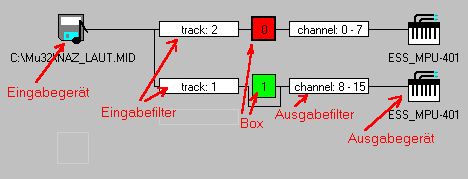
\includegraphics[width=234pt]{Route}
\fi
\end{center}

In diesem Fenster können Sie mit Doppelklick auf die einzelnen Icons
den zugehörigen Dialog zum Konfigurieren der Geräte und Routen öffnen.

Falls Sie \mutabor{} zu ersten mal starten, ist automatisch 
eine Konfiguration geladen, die Ihr erstes MIDI"=Eingabegerät 
mit dem ersten MIDI"=Ausgabegerät verbindet und alle Daten mutiert.

\begin{center}
\ifhtml
\HCode{<img src=\dq cc_route.png\dq  alt=\dq winecfg\dq   title=\dq winecfg\dq   width=\dq 443\dq  height=\dq 81\dq  class=\dq screenshot\dq   />}
\else
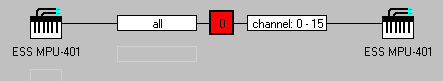
\includegraphics[width=221.5pt]{cc_route}
\fi
\end{center}

Sie können auch über das Menü "`Routes"' mit "`Load Routes"' eine
Konfiguration laden.

Genaueres zur Funktionsweise der Routen finden Sie im Abschnitt
\tsciteref{sec:DE_ROUTES}.


\helpsection{Logik-starten}{MANUAL_START_LOGIC}
\section{Logik  starten}
\label{sec:CC_LOGIC}

Hier wird erklärt, wie man ein \mutabor{}"=Programm übersetzen 
und starten kann. Zuvor sollten aber bereits die \reflink{sec:CC_CABLE}{MIDI"=Kabel}
angeschlossen und eine \reflink{sec:CC_ROUTES}{Route eingerichtet} haben.

\begin{enumerate}
\item Wählen Sie im \reflink{sec:DE_MENU}{Menü} unter
  "`\reflink{sec:MS_FILE}{File}"' den Punkt "`\reflink{sec:MI_OPEN}{Open}"'. Es
  erscheint ein (Ihnen sicher bekanntes) Dateiauswahl"=Fenster.
\item Doppelklicken Sie auf einer Datei, die das Anhängsel
  "`\texttt{.mut}"' hat, um diese Datei in den
  \reflink{sec:DE_EDIT}{Editor} zu laden (z.\,B.
  \texttt{Demo.mut}).
\item Danach wählen Sie im \reflink{sec:DE_MENU}{Menü} unter
  "`\reflink{sec:MS_LOGIC}{Logic}"' den Punkt
  "`\reflink{sec:MI_ACTIVATE}{Activate}"'.
\end{enumerate}

Darauf hin erscheint das \reflink{sec:DE_COMP}{Compiler"=Fenster} und
zeigt während der Programmübersetzung verschiedene Daten an.

Danach öffnet sich das \reflink{sec:DE_LOGIC}{Logiken"=Fenster}. Es enthält 
Symbole für Logiken und Umstimmungen. Diese können durch 
Mausklicks aktiviert werden.

Wenn Sie jetzt auf dem Keyboard spielen, werden die Töne entsprechende 
der angeklickten Logik verändert und mutiert.

\helpsection{MIDI--oder-Guido-Datei-abspielen}{MANUAL_PLAY_MIDI_OR_GUIDO_FILE}
\section{MIDI- oder Guido"=Datei abspielen}
\label{sec:CC_MIDIIN}


Hier wird erklärt, wie man eine \reflink{sec:DV_MIDIFILE}{MIDI"=Datei}
oder \reflink{sec:DV_GUIDO}{GUIDO"=Datei} unter \mutabor{} ganz normal 
abspielen kann. Zuvor sollten aber bereits die \reflink{sec:CC_CABLE}{MIDI"=Kabel} 
angeschlossen haben.


\begin{center}
\ifhtml
\HCode{<img src=\dq cc_midiin.png\dq  alt=\dq winecfg\dq   title=\dq winecfg\dq   width=\dq 471\dq  height=\dq 81\dq  class=\dq screenshot\dq   />}
\else
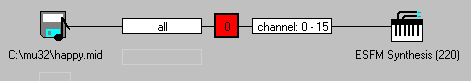
\includegraphics[width=235.5pt]{cc_midiin}
\fi
\end{center}

\begin{enumerate}
\item Klicken Sie im \reflink{sec:DE_MENU}{Menü} unter dem Punkt
  "`\reflink{sec:MS_VIEW}{View}"' auf
  "`\reflink{sec:MI_ROUTES}{Routes}"' um das
  "`\reflink{sec:DE_ROUTES}{Routenfenster}"' zu öffnen.
\item Mit einem Doppelklick auf das linke Symbol der
  Standardeinstellung bekommen sie die Möglichkeit das
  \reflink{sec:DE_R0}{"`Input"'"=Gerät} zu verändern!
\item Wählen sie das entsprechende Datei"=Format (MIDI oder Guido)!
\item Benutzen sie den Durchsuchen"=Knopf, wenn sie den genauen Ort
  der Datei nicht wissen
\item Wenn nun ein \tsreflink{Logikprogramm}{DV_LOGIKPROGRAMM}
  \reflink{sec:MI_ACTIVATE}{aktiviert} wird, erscheint links neben
  dem Datei"=Symbol ein Play- und ein Stop"=Knopf, mit dem sie das
  Abspielen der Dateien starten und beenden können.
\item Falls sie mehrere Dateien zugleich starten wollen, stehen Ihnen
  globale Play- und Stopknöpfe auf der
  \reflink{sec:DE_TOOLBAR}{Werkzeugleiste} oder im Menü
  "`\reflink{sec:MS_SEQUENCER}{Sequencer}"' zur Verfügung.
\end{enumerate}

Wichtig: Wenn Sie nun verschiedene Logiken aktivieren (und 
die Dateien durch eine entsprechende Box geleitet werden), \emph{wird 
die Musik der Eingabedatei entsprechend der aktuellen Logik mutiert}.



\helpsection{MIDI--oder-Guido-Datei-speichern}{MANUAL_SAVE_MIDI_OR_GUIDO}
\section{Ausgabe als MIDI- oder Guido"=Datei abspeichern}\label{sec:CC_MIDIOUT}




Ebenso wie Sie für die Eingabe eine Datei verwenden können, 
kann man auch für das Ausgabegerät eine Datei angeben. Die 
Daten werden dann nicht hörbar gemacht, sondern direkt in dieser 
Datei abgespeichert. Es empfiehlt sich dabei, eine parallele 
Route zu einem MIDI"=Gerät zu legen, damit man trotzdem hört 
was passiert.


\begin{center}
\ifhtml
\HCode{<img src=\dq cc_midiout.png\dq  alt=\dq winecfg\dq   title=\dq winecfg\dq   width=\dq 449\dq  height=\dq 136\dq  class=\dq screenshot\dq   />}
\else
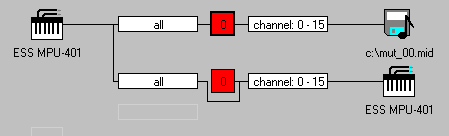
\includegraphics[width=224.5pt]{cc_midiout}
\fi
\end{center}

\begin{enumerate}
\item Klicken Sie im \reflink{sec:DE_MENU}{Menü} unter dem Punkt
  "`\reflink{sec:MS_VIEW}{View}"' auf
  "`\reflink{sec:MI_ROUTES}{Routes}"' um das
  \reflink{sec:DE_ROUTES}{Routenfenster} zu öffnen.
\item Mit einem Doppelklick auf das rechte Symbol der
  Standardeinstellung bekommen sie die Möglichkeit das
  \reflink{sec:DE_R4}{Ausgabe"=Gerät} zu verändern
\item Wählen sie das entsprechende Datei"=Format (MIDI oder Guido),
  und geben Sie einen Dateinamen für die neue Datei an.
\end{enumerate}


\paragraph{Parallele Route zum Anhören anlegen:} Doppelklicken Sie 
unterhalb des Eingabefilters im Routenfenster (z.\,B. in das hellgrau 
umrandete Feld). Es öffnet sich ein \reflink{sec:DE_R1}{Dialogfenster} 
für eine weitere Route. Stellen Sie ein, dass alle Daten durchgelassen 
werden. Doppelklicken Sie auf das Ende der Route. Es erscheint 
ein \reflink{sec:DE_R4}{Ausgabegerät"=Dialog} Dialog; stellen Sie in ihm 
ihr MIDI"=Gerät oder die Soundkarte ein, damit Sie hören können, 
welche Daten in die Datei geleitet werden.

\begin{center}
\ifhtml
\HCode{<img src=\dq cc_midioutpara.png\dq  alt=\dq winecfg\dq   title=\dq winecfg\dq   width=\dq 453\dq  height=\dq 130\dq  class=\dq screenshot\dq   />}
\else
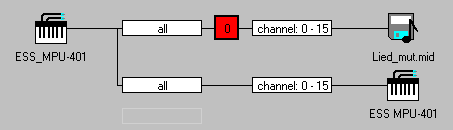
\includegraphics[width=226.5pt]{cc_midioutpara}
\fi
\end{center}

\helpsection{Bedienelemente}{MANUAL_WIDGETS}
\part{Die Bedienelemente von \mutabor}

\helpsection{Hauptfenster}{MANUAL_MAINWINDOW}
\chapter{Hauptfenster}\label{sec:DE_MAINWINDOW}

Nach dem Programmstart meldet sich \mutabor{} mit dem Hauptfenster.
Dieses ist in mehrere Zonen eingeteilt. Außen herum befindet sich
meist ein Fensterrahmen, der am oberen Rand etwas dicker ist und den
Titel des Fensters (hier "`\mutabor"') anzeigt. Ob und wie dieser
Rahmen angezeigt hängt nicht von \mutabor{}, sondern vielmehr von den
Einstellungen der Grafischen Oberfläche Ihres Computer"=Systems ab.
Darauf folgen die \reflink{sec:DE_MENU}{Menüleiste}, die
\reflink{sec:DE_TOOLBAR}{Werkzeugleiste}, der Bereich für die
\reflink{sec:DE_SUBWINDOW}{Unterfenster} und die
\reflink{sec:DE_STATUS}{Statusleiste}.

\helpsection{Werkzeugleiste}{MANUAL_TOOLBAR}
\section{Werkzeugleiste}\label{sec:DE_TOOLBAR}
Die Werkzeugleiste befindet sich unmittelbar unterhalb des Menüs.
Durch Klicken auf ihre Piktogramme können Sie einige häufig gebrauchte
Befehle schneller ausführen.

\helpsection{Statusleiste}{MANUAL_STATUS_BAR}
\section{Statusleiste}\label{sec:DE_STATUS}
Die Statusleiste befindet sich am unteren Rand des Programm"=Fensters.
Hier können Sie sehen, ob der Editor gerade im überschreiben- oder
Einfügen"=Modus arbeitet und hier werden auch die Flyover"=Hints
angezeigt. Ein Piktogramm informiert, ob ein
\reflink{sec:DV_LOGIKPROGRAMM}{Logikprogramm} aktiviert ist, in diesem
Fall, wird hier auch die \reflink{sec:DV_CURRENTBOX}{aktuelle Box} die
aktuelle Logik mit dem gegenwärtigen Tonsystem angezeigt.


\helpsection{Menueleiste}{MANUAL_MENUBAR}
\chapter{Menüleiste}
\label{sec:DE_MENU}
Die Umgebung von \mutabor{} bietet Ihnen alle Funktionen, die Sie zum
Schreiben, Editieren, übersetzen, Ausführen und Verwalten Ihrer
\mutabor{}"=Programme benötigen. Durch die Menüzeile am oberen Rand
des Desktop haben Sie Zugriff auf die Menüs.

Die Menüzeile wird durch die Funktionstaste \keystroke{F10} oder mit der 
Maus durch Klicken auf den entsprechenden Bereich aktiviert.

Die Menüzeile enthält die folgenden Befehle:
\begin{description}
\item[\tsreflink{File}{MS_FILE}] Dateiverwaltung, Optionen
\item[\tsreflink{Edit}{MS_EDIT}] Editier"=Funktionen für Quelltexte
\item[\tsreflink{Search}{MS_SEARCH}] Suchen im Quelltext
\item[\tsreflink{Logic}{MS_LOGIC}] Arbeiten mit Logiken
\item[\tsreflink{Routes}{MS_ROUTES}] Routenverwaltung
\item[\tsreflink{View}{MS_VIEW}] Anzeigeelemente anzeigen oder verbergen
\item[\tsreflink{Sequencer}{MS_SEQUENCER}] Sequenzer"=Funktionen
\item[\tsreflink{Window}{MS_WINDOW}] Fensterverwaltung
\item[\tsreflink{Help}{MS_HELP}] Hilfe anzeigen, Versionsinformation
\end{description}

\helpsection{Datei-Oeffnen-Speichern}{MANUAL_FILE_OPEN_SAVE}
\section{Datei öffnen, speichern\texorpdfstring\dots{...}}
\label{sec:MS_FILE}

Das Menü "`Datei"' beinhaltet Befehle zum Anlegen neuer Dateien, 
öffnen bestehender Dateien, Speichern und direktem Ausführen 
von \mutabor{}"=Dateien sowie zum Verlassen von \mutabor{}. 
Außerdem kann man hier einige globale Optionen einstellen.


\begin{description}
\item[\reflink{sec:MI_NEW}{New}] Neue Datei
\item[\reflink{sec:MI_OPEN}{Open}] Datei öffnen
\item[\reflink{sec:MI_SAVE}{Save}] Datei abspeichern
\item[\reflink{sec:MI_SAVEAS}{Save as}] Datei speichern unter\dots
\item[\reflink{sec:MI_EXECUTE}{Execute}] Datei direkt ausführen
\item[\reflink{sec:MI_SETUP}{Options}] Globale Einstellungen
\item[\reflink{sec:MI_EXIT}{Exit}] \mutabor{} verlassen
\end{description}


\helpsection{Neue-Datei}{MANUAL_FILE_NEW}
\subsection{Neue Datei}\label{sec:MI_NEW}
Dieser Befehl öffnet ein neues Editorfenster mit dem voreingestellten
Namen "`UNTITLED"' und aktiviert automatisch dieses neue Editorfenster.
Dort können sie dann einen neuen Programm"=Text eingeben. Diese
UNTITLED"=Dateien dienen als temporäre Puffer des Editors.  Beim
Speichern werden Sie aufgefordert, einen neuen Namen zu vergeben.

\helpsection{Datei-oeffnen}{MANUAL_FILE_OPEN}
\subsection{Datei öffnen}
\label{sec:MI_OPEN}

Dieser Befehl öffnet eine \reflink{sec:DV_QUELLTEXT}{Quelltext"=Datei}
und lädt sie in ein \reflink{sec:DE_EDIT}{Editor"=Fenster}. Dazu
erscheint ein übliches Dateiauswahl"=Fenster. In diesem können Sie die
gewünschte Datei auswählen; klicken Sie danach auf "`OK"' oder brechen Sie
den Vorgang ab.


\helpsection{Datei-speichern}{MANUAL_FILE_SAVE}
\subsection{Datei abspeichern}\label{sec:MI_SAVE}
Dieser Befehl sichert den \reflink{sec:DV_QUELLTEXT}{Quelltext} des gerade 
aktiven \reflink{sec:DE_EDIT}{Editor"=Fensters} auf Diskette oder Festplatte. 
Wenn noch kein Name angegeben wurde, werden Sie zuvor zur Angabe 
eines Namens für die Datei aufgefordert.


\helpsection{Datei-speichern-unter}{MANIAL_FILE_SAVE_AS}
\subsection{Datei abspeichern unter\dots{}}\label{sec:MI_SAVEAS}

Dieser Befehl öffnet ein Dateiauswahl"=Fenster, mit dessen Hilfe Sie
den \reflink{sec:DV_QUELLTEXT}{Quelltext} aus dem aktiven
\reflink{sec:DE_EDIT}{Editor"=Fenster} unter einem anderen Namen und
in einem anderen Verzeichnis oder Laufwerk speichern können.


Geben Sie den neuen Namen ein, optional Verzeichnis und/""oder Laufwerk,
und klicken oder wählen Sie "`OK"'. Die Namen aller Editorfenster mit
dieser Datei werden automatisch umbenannt.


Wenn Sie einen vorhandenen Dateinamen verwenden, fragt \mutabor{}, ob
die Datei überschrieben werden soll.


\helpsection{Datei-ausfuehren}{MANUAL_FILE_EXECUTE}
\subsection{Datei direkt ausführen}
\label{sec:MI_EXECUTE}

Mit diesem Befehl können Sie eine Datei als \mutabor{}"=Programm
ausführen, ohne sie zuvor in ein Editorfenster zu laden. Es öffnet
sich ein Dateiauswahl"=Fenster.


Wählen Sie in diesem die gewünschte Quelldatei und wählen "`OK"'. Die
Datei wird daraufhin compiliert, es erscheint (bei fehlerfreier
Übersetzung) das \reflink{sec:DE_LOGIC}{Logiken"=Fenster} und das
Programm ist aktiviert.

\helpsection{Datei-Einstellungen}{MANUAL_FILE_SETTINGS}
\subsection{Optionen"=Dialog aufrufen}\label{sec:MI_SETUP}

Dieser Befehl öffnet den \reflink{sec:DE_SETUP}{Optionen"=Dialog}, in 
dem Sie einige globale Parameter für \mutabor{} einstellen 
können.

\helpsection{Beenden}{MANUAL_FILE_QUIT}
\subsection{\mutabor{} beenden}
\label{sec:MI_EXIT}

Dieser Befehl beendet die Arbeit mit \mutabor{}. Wenn sich noch nicht
gespeicherte Quelltexte im Editor befinden, wird abgefragt, ob jene
gespeichert werden sollen.


\helpsection{Editierfunktionen}{MANUAL_EDIT_FUNCTIONS}
\section{Editierfunktionen}\label{sec:MS_EDIT}
Das Menü "`Edit"' beinhaltet Befehle zum Bearbeiten des Textes 
in den \reflink{sec:DE_EDIT}{Editor"=Fenstern}.

\begin{description}
\item[\reflink{sec:MI_UNDO}{Undo}] Rückgängig
\item[\reflink{sec:MI_CUT}{Cut}] Ausschneiden
\item[\reflink{sec:MI_COPY}{Copy}] Kopieren
\item[\reflink{sec:MI_PASTE}{Paste}] Einfügen
\item[\reflink{sec:MI_DELETE}{Delete}] Löschen
\item[\reflink{sec:MI_CLEAR}{Clear All}] Alles löschen
\end{description}

\helpsection{Rueckgaengig}{MANUAL_EDIT_UNDO}
\subsection{Rückgängig}
\label{sec:MI_UNDO}

Der Befehl Rückgängig macht die letzten Eingaben oder Cursorbewegungen
rückgängig. Gelöschte Zeichen werden eingefügt, eingefügte gelöscht,
überschriebene Zeichen restauriert und der Cursor auf die alte
Position zurückgesetzt. Wenn Sie eine Blockoperation zurücknehmen,
erscheint Ihre Datei wie vor der Ausführung des Blockbefehls. Wenn Sie
den Befehl wiederholt geben, werden nacheinander die Änderungen an der
Datei zurückgenommen, die seit dem Öffnen vorgenommen wurden.

\helpsection{Ausschneiden}{MANUAL_EDIT_CUT}
\subsection{Ausschneiden}\label{sec:MI_CUT}
Der Befehl "`Cut"' entfernt den markierten Text aus dem aktiven
\reflink{sec:DE_EDIT}{Editor"=Fenster} und kopiert ihn in
die Zwischenablage. Mit dem Befehl \reflink{sec:MI_PASTE}{Einfügen}
können Sie diesen Text in ein anderes Fenster (oder an eine andere
Stelle im selben Fenster) kopieren.

Der Text bleibt in der Zwischenablage, so dass man ihn beliebig 
oft kopieren kann. 


\helpsection{Kopieren}{MANUAL_EDIT_COPY}
\subsection{Kopieren}\label{sec:MI_COPY}
Copy kopiert den markierten Text aus dem aktiven
\reflink{sec:DE_EDIT}{Editor"=Fenster} in die Zwischenablage, ohne ihn
aus dem Fenster zu löschen.

Mit \reflink{sec:MI_PASTE}{Einfügen} können Sie diesen Text in ein 
anderes Fenster (oder an eine andere Stelle im selben Fenster) 
kopieren.  

Sie können auch Text (z.\,B. Beispiele) aus einem Hilfefenster 
kopieren. Drücken Sie die Umschalt- und eine Pfeiltaste, um 
den Text zu markieren. Wählen Sie anschließend Kopieren, 
um ihn in die Zwischenablage zu kopieren. Mit der Maus können 
Sie den Text selektieren und ihn anschließend an die gewünschte 
Stelle ziehen.

\helpsection{Einfuegen}{MANUAL_EDIT_INSERT}
\subsection{Einfügen}
\label{sec:MI_PASTE}

Dieser Befehl fügt den in der Zwischenablage markierten Text 
an der Cursorposition im aktiven Editor"=Fenster ein.

\helpsection{Loeschen}{MANUAL_EDIT_DELETE}
\subsection{Löschen}
\label{sec:MI_DELETE}
"`Delete"' löscht den markierten Text, ohne ihn in die Zwischenablage 
zu kopieren.


Dieser Text ist nicht mehr rekonstruierbar und steht für Einfügeoperationen 
nicht zur Verfügung. Benutzen Sie hierfür "`\reflink{sec:MI_CUT}{Ausschneiden}"'
oder "`\reflink{sec:MI_COPY}{Kopieren}"'.


Sie können zwar den gelöschten Text nicht mehr kopieren, aber den
Löschbefehl mit "`\reflink{sec:MI_UNDO}{Rückgängig}"' rückgängig
machen.

Löschen ist dann nützlich, wenn Sie Text löschen, aber 
den in der Zwischenablage befindlichen Text nicht überschreiben 
wollen.

\helpsection{Alles-loeschen}{MANUAL_EDIT_DELETEALL}
\subsection{Alles löschen}
\label{sec:MI_CLEAR}
Mit diesem Befehl löschen Sie den gesamten Inhalt des aktuellen 
Editor"=Fensters.



\helpsection{Textsuche}{MANUAL_TEXT_SEARCH}
\section{Suchen im Text}\label{sec:MS_SEARCH}
Das Menü Search beinhaltet Befehle zum Suchen und Ersetzen 
von Text in den \reflink{sec:DE_EDIT}{Editor"=Fenstern}.

\begin{description}
\item[\reflink{sec:MI_FIND}{Search}] Suchen
\item[\reflink{sec:MI_REPLACE}{Replace}] Ersetzen
\item[\reflink{sec:MI_NEXT}{Next}] Weitersuchen
\end{description}

\helpsection{Suchen}{MANUAL_EDIT_SEARCH}
\subsection{Suchen}
\label{sec:MI_FIND}

Dieser Befehl zeigt das Dialogfenster zum Suchen von Text im 
aktiven \reflink{sec:DE_EDIT}{Editor"=Fenster} an. Geben Sie den Begriff, 
nach dem Sie suchen möchten, ein. Weiterhin können Sie mehrere 
Optionen angeben, die die Suche beeinflussen.


Anschließend wird der Quelltext nach dem angegebenen Wort durchsucht,
der Begriff wird als markierter Text dargestellt. Mit
\reflink{sec:MI_NEXT}{Suche/""Ersetzen wiederholen} können Sie die Suche
gegebenenfalls fortsetzen.


\helpsection{Replace}{MANUAL_EDIT_REPLACE}
\subsection{Ersetzen}\label{sec:MI_REPLACE}

Dieser Befehl öffnet ein Dialogfenster zum Ersetzen von Text 
im Quelltext, in das Sie den Text, der gesucht, und den Text, 
der den gefundenen Begriff ersetzen soll, eingeben können. 
Weiterhin können Sie mehrere Optionen angeben, die die Suche 
beeinflussen. Anschließend wird der Quelltext nach dem angegebenen 
Wort durchsucht und dieser wird durch den angegebenen Text ersetzt. 
Mit \reflink{sec:MI_NEXT}{Suche/""Ersetzen wiederholen} können Sie den 
Vorgang gegebenenfalls fortsetzen.

\helpsection{Weitersuchen}{MANUAL_EDIT_SEARCH_AGAIN}
\subsection{Suche/""Ersetzen wiederholen}
\label{sec:MI_NEXT}

Dieser Befehl wiederholt den letzten "`\reflink{sec:MI_FIND}{Suchen-}"'
oder \reflink{sec:MI_REPLACE}{"`Ersetzen"'"=Befehl}.



Alle Einstellungen, die Sie in den Dialogfenstern Suchen nach 
Text und Text ersetzen vorgenommen haben, werden bei der Ausführung 
des Befehls verwendet. 


\helpsection{Logik-compilieren-starten}{MANUAL_COMPILE_START_LOGIC}
\section{Logik compilieren, starten\dots}\label{sec:MS_LOGIC}

Das Menü "`Logic"' beinhaltet Befehle zum übersetzen, Aktivieren 
und Anhalten eines Logikprogramms sowie eine All"=Note"=Off"=Funktion.


\begin{description}
\item[\reflink{sec:MI_COMPILE}{Compile}]
  \reflink{sec:DV_LOGIKPROGRAMM}{Logikprogramm} übersetzen
\item[\reflink{sec:MI_ACTIVATE}{Activate}]
  \reflink{sec:DV_LOGIKPROGRAMM}{Logikprogramm} aktivieren
\item[\reflink{sec:MI_STOP}{Stop}]
  \reflink{sec:DV_LOGIKPROGRAMM}{Logikprogramm} anhalten 
\item[\reflink{sec:MI_PANIC}{Panic}] Alle klingenden Töne ausschalten
\end{description}

\helpsection{Logik-Uebersetzen}{MANUAL_LOGIC_COMPILE}
\subsection{Programm übersetzen}
\label{sec:MI_COMPILE}


Dieser Menüeintrag startet den Compiler, der den
\reflink{sec:DV_QUELLTEXT}{Quelltext} des aktuellen
\reflink{sec:DE_EDIT}{Editor"=Fensters} übersetzt. Dabei wird das
\reflink{sec:DE_COMP}{Compiler"=Fenster} mit verschiedenen
statistischen Daten zum \reflink{sec:DV_LOGIKPROGRAMM}{Logikprogramm}
angezeigt. Wenn der Compiler Fehler im Programmtext findet, so zeigt
er die an, ansonsten meldet er die fehlerfreie Übersetzung.

\helpsection{Logik-Ausfuehren}{MANUAL_LOGIC_EXECUTE}
\subsection{Programm ausführen}
\label{sec:MI_ACTIVATE}

Mit diesem Menüeintrag veranlassen Sie die Übersetzung des
\reflink{sec:DV_QUELLTEXT}{Quelltextes} des aktuellen
\reflink{sec:DE_EDIT}{Editorfensters} und (bei fehlerfreier
Übersetzung) die Aktivierung des
\reflink{sec:DV_LOGIKPROGRAMM}{Logikprogramms}. Dazu öffnet sich das
\reflink{sec:DE_LOGIC}{Logiken"=Fenster} und die jeweils aktivierten
\reflink{sec:DV_PROTOKOLL}{Protokoll"=Fenster}. Sie können nun mit den
Logiken arbeiten, d.\,h. auf dem angeschlossenen Keyboard spielen,
\reflink{sec:DV_MIDIFILE}{MIDI"=Dateien} abspielen usw.  Diesen
Arbeitsmodus können Sie durch das \reflink{sec:MI_STOP}{Stoppen} der
Logiken wieder beenden.

\helpsection{Batchmodus}{MANUAL_LOGIC_BATCH_MODE}
\subsection{Batch"=Modus}


Wenn Sie in den Route nur \reflink{sec:DV_MIDIFILE}{MIDI"=Dateien} verwendet 
haben, bietet \mutabor{} Ihnen an, das ganze im sogenannten 
Batch Modus auszuführen. Dabei werden die Dateien beim Drücken 
des \reflink{sec:MI_INDEVPLAY}{Play"=Knopfes} auf einen Schlag übersetzt. 
Die Ausgabedateien verwenden dann exakt das gleiche Zeitformat 
(Speed, Ticks usw.) wie die Eingabedateien. Bei dieser Art der 
Übersetzung ist es natürlich nicht möglich, direkt während 
des Abspielens über Computertastatur die Logiken zu beeinflussen 
(wohl aber über die Harmonieanalyse). Die Anfangslogiken/""Stimmungen 
stellt man wie gewöhnlich \emph{vor} Drücken des \reflink{sec:MI_INDEVPLAY}{Play"=Knopfes} 
ein.

\subsubsection{Motivation/""Technischer Hintergrund}


Im live"=Betrieb spielt \mutabor{} die MIDI"=Dateien Zeitraster 
von 2 Millisekunden ab. Die Ausgabe"=MIDI"=Dateien verwenden dies 
dann ebenfalls und haben daher eine etwas ungewöhnliche time 
base und leiden zusätzlich z.\,T. unter den Rundungsfehlern. 
Beim Batch Modus hingegen werden die originalen Timing"=Daten 
verwendet.


Da man sich die Dateien im Batch Modus nicht anhören kann, 
empfiehlt es sich, die Dateien beim Experimentieren zunächst 
auf ein MIDI"=Gerät auszugeben (zum hören), und erst dann, 
wenn man ein befriedigendes Ergebnis erreicht hat, die Eingabedateien 
im Batch Modus in Ausgabedateien zu übernehmen (zum weiterverarbeiten).


\helpsection{Programm-stoppen}{MANUAL_LOGIC_STOP}
\subsection{Programm stoppen}\label{sec:MI_STOP}



Hiermit können Sie ein \reflink{sec:DV_LOGIKPROGRAMM}{Logikprogramm},
das Sie \reflink{sec:MI_ACTIVATE}{aktiviert} haben, wieder stoppen. Das 
ist notwendig, wenn Sie eine andere Logik aktivieren oder sich 
eine \reflink{sec:DV_MIDIFILE}{MIDI"=Datei} \textit{unmutiert} anhören wollen.


\helpsection{Panik}{MANUAL_PANIC}
\subsection{Panik"=Funktion}\label{sec:MI_PANIC}



Wenn Sie diesen Befehl auslösen, wird an die MIDI"=Ausgabegeräte 
ein ``All"=Note"=Off''"=Befehl gesendet, der alle gerade klingenden 
Töne abschaltet. Dies kann notwendig sein, wenn irgendwelche 
Töne ``hängen geblieben'' sind.



\helpsection{Routen-laden-und-speichern}{MANUAL_LOAD_SAVE_ROUTES}
\section{Routen laden und speichern}\label{sec:MS_ROUTES}
Im Menü "`Routes"' können sie Routen"=Konfigurationen laden 
und speichern.

\begin{description}
\item[\reflink{sec:MI_ROUTELOAD}{Load Routes}] Routen laden
\item[\reflink{sec:MI_ROUTESAVE}{Save Routes}] Routen abspeichern
\item[\reflink{sec:MI_ROUTESAVEAS}{Save Routes as}] Routen unter neuem
  Dateinnamen abspeichern
\end{description}

\helpsection{Route-laden}{MANUAL_ROUTE_LOAD}
\subsection{Routen laden}\label{sec:MI_ROUTELOAD}


Dieser Befehl öffnet eine \reflink{sec:DV_ROUTESFILE}{Routen"=Datei} 
und lädt sie in das \reflink{sec:DE_ROUTES}{Routen"=Fenster}. Dazu erscheint 
ein übliches Dateiauswahl"=Fenster. In diesem können Sie die 
gewünschte Datei auswählen; klicken Sie danach auf "`OK"' oder 
brechen Sie den Vorgang ab.


\helpsection{Route-speichern}{MANUAL_ROUTE_SAVE}
\subsection{Routen abspeichern}\label{sec:MI_ROUTESAVE}



Dieser Befehl sichert den Inhalt des \reflink{sec:DE_ROUTES}{Routen"=Fensters} 
auf Diskette oder Festplatte in Form einer \reflink{sec:DV_ROUTESFILE}{Routen"=Datei}. 
Wenn noch kein Name angegeben wurde, werden Sie zuvor zur Angabe 
eines Namens für die Datei aufgefordert.


\helpsection{Route-speichern-unter}{MANUAL_ROUTE_SAVE_AS}
\subsection{Routen abspeichern unter \dots}\label{sec:MI_ROUTESAVEAS}



Dieser Befehl öffnet ein Dateiauswahl"=Fenster, mit dessen Hilfe Sie
den Inhalt des \reflink{sec:DE_ROUTES}{Routen"=Fensters} als
\reflink{sec:DV_ROUTESFILE}{Routen"=Datei} unter einem anderen Namen
und in einem anderen Verzeichnis oder Laufwerk speichern können.


Geben Sie den neuen Namen ein, optional Verzeichnis und/""oder 
Laufwerk, und klicken oder wählen Sie "`OK"'.


Wenn Sie einen vorhandenen Dateinamen verwenden, fragt \mutabor{}, 
ob die Datei überschrieben werden soll. 


\helpsection{Dialogelemente-anzeigen}{MANUAL_SHOW_DIALOG_ELEMENTS}
\section{Anzeigen verschiedener Dialogelemente}\label{sec:MS_VIEW}
Im Menü "`View"' können sie auswählen, welche Fenster und 
Dialogelemente angezeigt werden sollen.

\begin{description}
\item[\reflink{sec:MI_STATUS}{Statusbar}]
  \reflink{sec:DE_STATUS}{Statusleiste} einblenden/""ausblenden
\item[\reflink{sec:MI_TOOLBAR}{Toolbar}]
  \reflink{sec:DE_TOOLBAR}{Werkzeugleiste} einblenden/""ausblenden
\item[\reflink{sec:MI_ROUTES}{Routes}]
  \reflink{sec:DE_ROUTES}{Routen"=Fenster} anzeigen
\item[\reflink{sec:MI_KEY}{Current Keys}]
  \reflink{sec:DE_KEY}{Aktuelle"=Tasten"=Fenster} einblenden/""ausblenden
\item[\reflink{sec:MI_TS}{Tone System}]
  \reflink{sec:DE_TS}{Tonsystem"=Fenster} einblenden/""ausblenden
\item[\reflink{sec:MI_ACTION}{Actions}]
  \reflink{sec:DE_ACTION}{Aktionsfenster} einblenden/""ausblenden
\item[\reflink{sec:MI_OWM}{One window mode}]
  \reflink{sec:DV_OWM}{"`Ein"=Fenster"'"=Modus} aktivieren/""deaktivieren
\item[\reflink{sec:MI_CAW}{One common action window}]
  \reflink{sec:DV_CAW}{"`Gemeinsames Aktionen"=Fenster"'"=Modus}
  aktivieren/""deaktivieren
\item[\reflink{sec:MI_SELECTBOX}{Select box}]
  \reflink{sec:DV_CURRENTBOX}{Aktuelle Box} auswählen
\end{description}

\helpsection{Werkzeugleiste-ein-ausblenden}{MANUAL_SWITCH_TOOLBAR}
\subsection{Werkzeugleiste ein"=/""ausblenden}
\label{sec:MI_TOOLBAR}

Mit diesem Menüeintrag können Sie auswählen, ob die
\reflink{sec:DE_TOOLBAR}{Werkzeugleiste} angezeigt werden soll oder
nicht.


\helpsection{Statusleiste-ein-ausblenden}{MANUAL_SWITCH_STATUSBAR}
\subsection{Statusleiste ein"=/""ausblenden}
\label{sec:MI_STATUS}

Mit diesem Menüeintrag können Sie auswählen, ob die \reflink{sec:DE_STATUS}{Statusleiste} 
angezeigt werden soll oder nicht.


\helpsection{Routenfenster-anzeigen}{MANUAL_SHOW_ROUTES}
\subsection{Routen"=Fenster anzeigen}\label{sec:MI_ROUTES}


Dieser Befehl zeigt das \reflink{sec:DE_ROUTES}{Routen"=Fenster} an bzw. 
zeigt es als oberstes Fenster.


\helpsection{Aktuelle-Tasten-ein-ausbelenden}{MANUAL_SHOW_CURRENT_KEYS}
\subsection{"`Aktuelle"=Tasten"'"=Fenster ein"=/""ausblenden}\label{sec:MI_KEY}
Mit diesem Menüeintrag können Sie auswählen, ob das
\reflink{sec:DE_KEY}{Aktuelle"=Tasten"=Fenster} der gerade
\reflink{sec:DV_CURRENTBOX}{aktuellen Box} angezeigt werden soll oder
nicht. Wenn der \reflink{sec:DV_OWM}{"`Ein"=Fenster"'"=Modus}
aktiviert ist handelt es sich dabei allgemeine
\reflink{sec:DE_KEY}{Aktuelle"=Tasten"=Fenster} für alle Boxen


\helpsection{Tonsystemfenster-ein-ausblenden}{MANUAL_SHOW_TONE_SYSTEM}
\subsection{Tonsystem"=Fenster ein"=/""ausblenden}
\label{sec:MI_TS}
Mit diesem Menüeintrag können Sie auswählen, ob das
\reflink{sec:DE_TS}{Tonsystem"=Fenster} der gerade
\reflink{sec:DV_CURRENTBOX}{aktuellen Box} angezeigt werden soll oder
nicht. Wenn der \reflink{sec:DV_OWM}{"`Ein"=Fenster"'"=Modus}
aktiviert ist handelt es sich dabei allgemeine
\reflink{sec:DE_TS}{Tonsystem"=Fenster} für alle Boxen.


\helpsection{Aktionsfenster-ein-ausblenden}{MANUAL_SHOW_ACTION_WINDOW}
\subsection{Aktionen"=Fenster ein"=/""ausblenden}
\label{sec:MI_ACTION}

Mit diesem Menüeintrag können Sie auswählen, ob das
\reflink{sec:DE_ACTION}{Aktionen"=Fenster} der gerade
\reflink{sec:DV_CURRENTBOX}{aktuellen Box} angezeigt werden soll oder
nicht.


Wenn der \reflink{sec:DV_OWM}{"`Ein"=Fenster"'"=Modus} aktiviert 
ist handelt es sich dabei \reflink{sec:DE_ACTION}{Aktionen"=Fenster} für 
alle Boxen, wenn der \reflink{sec:DV_CAW}{"`Gemeinsames Aktionen"=Fenster"'"=Modus}
aktiviert ist handelt es sich um das gemeinsame \reflink{sec:DE_ACTION}{Aktionen"=Fenster} 
für alle Boxen.

\helpsection{Ein-Fenster-Modus-aktivieren}{MANUAL_ONE_WINDOW_MODE}
\subsection{"`Ein"=Fenster"'"=Modus aktivieren/""deaktivieren}
\label{sec:MI_OWM}
Mit diesem Menüeintrag können den \reflink{sec:DV_OWM}{"`Ein"=Fenster"'"=Modus}
ein- und ausschalten.


Ist dieser Modus aktiviert, so gibt es jedes
\reflink{sec:DV_PROTOKOLL}{Protokoll"=Fenster} nur in einer
Ausführung. In diesen werden die Daten der
\reflink{sec:DV_CURRENTBOX}{gerade aktuellen Box} angezeigt. Wird eine
andere Box als aktuelle \reflink{sec:MI_SELECTBOX}{Box ausgewählt}, so
ändert sich automatisch der Inhalt der Protokollfenster. Dies gewährt
eine gewisse Übersichtlichkeit, da die Fensteranzahl begrenzt ist.


Ist dieser Modus nicht aktiviert, so hat jede Box ihre eigenen
\reflink{sec:DV_PROTOKOLL}{Protokoll"=Fenster}. Sie können so z.\,B.
mehrere \reflink{sec:DE_KEY}{Aktuelle"=Tasten"=Fenster} verschiedener
Boxen parallel anzeigen lassen und deren Inhalte vergleichend
verfolgen.


\helpsection{Gemeinsame-Aktionen}{MANUAL_COMMON_ACTION_WINDOW}
\subsection{"`Gemeinsames Aktionen"=Fenster"'"=Modus aktivieren/""deaktivieren}
\label{sec:MI_CAW}
Mit diesem Menüeintrag können den \reflink{sec:DV_CAW}{"`Gemeinsames
  Aktionen"=Fenster"'"=Modus} ein- und ausschalten.


Ist dieser Modus aktiviert, so gibt es nur ein
\reflink{sec:DE_ACTION}{Aktionen"=Fenster}, in dem die Aktionen aller
Boxen angezeigt werden. Dazu wird vor jeder Aktion die Nummer der Box
angegeben.


Ist dieser Modus nicht aktiviert, so hat jede Box ihre eigenes
\reflink{sec:DE_ACTION}{Aktionen"=Fenster}, dem nur die Aktionen
dieser Box angezeigt werden. Ist in diesem Fall der
\reflink{sec:DV_OWM}{"`Ein"=Fenster"'"=Modus}aktiviert, so wird zwar
auch nur ein Aktionen"=Fenster angezeigt, dieses zeigt aber auch nur
die Aktionen der gerade \reflink{sec:DV_CURRENTBOX}{aktuellen Box}.


\helpsection{Box-auswaehlen}{MANUAL_SELECT_BOX}
\subsection{Aktuelle Box auswählen}
\label{sec:MI_SELECTBOX}

Dieser Eintrag öffnet bei aktivierten
\reflink{sec:DV_LOGIKPROGRAMM}{Logikprogramm} ein Menü, in dem Sie die
\reflink{sec:DV_CURRENTBOX}{aktuelle Box} auswählen können. Klicken
Sie dazu auf die entsprechenden Eintrag. Die gerade aktuelle Box ist
mit einem Haken markiert.


\helpsection{Sequenzer-bedienen}{MANUAL_SEQUENCER}
\section{Sequenzer bedienen}\label{sec:MS_SEQUENCER}
Das Menü "`Sequencer"' beinhaltet Befehle zum synchronen Starten 
und Stoppen der Eingabegeräte im \reflink{sec:DE_ROUTES}{Routen"=Fenster}. 
Um einzelne Dateien separat zu starten verwenden Sie die Startknöpfe 
neben den Dateisymbolen im \reflink{sec:DE_ROUTES}{Routen"=Fenster} .

\begin{description}
\item[\reflink{sec:MI_INDEVPLAY}{Play}] Abspielen starten
\item[\reflink{sec:MI_INDEVSTOP}{Stop}] Abspielen abbrechen
\item[\reflink{sec:MI_INDEVPAUSE}{Pause}] Abspielen anhalten (Pause)
\end{description}

\helpsection{Sequenzer-starten}{MANUAL_START_SEQUENCER}
\subsection{Sequenzer starten}
\label{sec:MI_INDEVPLAY}


Dieser Befehl startet synchron das Abspielen aller Dateien, die im
\reflink{sec:DE_ROUTES}{Routes"=Fenster} als Eingabegeräte
eingerichtet sind. Falls Geräte vorher nur angehalten wurden, setzen
sie das Abspielen an genau dieser Stelle wieder fort.


Alternativ dazu befinden sich im
\reflink{sec:DE_ROUTES}{Routes"=Fenster} bei
\reflink{sec:MI_ACTIVATE}{aktiviertem}
\reflink{sec:DV_LOGIKPROGRAMM}{Logikprogramm} an jedem
Datei"=Eingabegerät kleinen Knöpfe, mit denen das Abspielen gesteuert
werden kann.


\helpsection{Sequenzer-stoppen}{MANUAL_STOP_SEQUENCER}
\subsection{Sequenzer abbrechen}\label{sec:MI_INDEVSTOP}


Dieser Befehl beendet das Abspielen aller Dateien, die im
\reflink{sec:DE_ROUTES}{Routes"=Fenster} als Eingabegeräte
eingerichtet sind.


Alternativ dazu befinden sich im
\reflink{sec:DE_ROUTES}{Routes"=Fenster} bei
\reflink{sec:MI_ACTIVATE}{aktiviertem}
\reflink{sec:DV_LOGIKPROGRAMM}{Logikprogramm} an jedem
Datei"=Eingabegerät kleinen Knöpfe, mit denen das Abspielen gesteuert
werden kann.


\helpsection{Sequenzer-pausieren}{MANUAL_PAUSE_SEQUENCER}
\subsection{Sequenzer vorübergehend anhalten}
\label{sec:MI_INDEVPAUSE}

Dieser Befehl startet unterbricht synchron das Abspielen aller
Dateien, die im \reflink{sec:DE_ROUTES}{Routes"=Fenster} als
Eingabegeräte eingerichtet sind. Sie können das Abspielen fortsetzen
in dem Sie im \reflink{sec:DE_MENU}{Menü}
\reflink{sec:MS_SEQUENCER}{Sequencer} auf
\reflink{sec:MI_INDEVPLAY}{Play} klicken (alle Dateien synchron) oder
einzeln über die Knöpfe im \reflink{sec:DE_ROUTES}{Routes"=Fenster}.


Alternativ dazu befinden sich im
\reflink{sec:DE_ROUTES}{Routes"=Fenster} bei
\reflink{sec:MI_ACTIVATE}{aktiviertem}
\reflink{sec:DV_LOGIKPROGRAMM}{Logikprogramm} an jedem
Datei"=Eingabegerät kleinen Knöpfe, mit denen das Abspielen gesteuert
werden kann.

\iffalse  % gibts nicht mehr
\helpsection{Fensterfunktionen}{MANUAL_WINDOW_FUNCTIONS}
\section{Fensterfunktionen}\label{sec:MS_WINDOW}
Das Menü "`Windows"' enthält Befehle um die Fenster übereinander 
oder nebeneinander darzustellen, die ionisierten Fenster anzuordnen 
oder alle Fenster zu schließen.

\begin{description}
\item[\reflink{sec:MI_CASCADE}{Cascade}] Fenster hintereinander
\item[\reflink{sec:MI_TILE}{Tile}] Fenster nebeneinander
\item[\reflink{sec:MI_ARRANGEICONS}{Arrange Icons}] Icons anordnen
\item[\reflink{sec:MI_CLOSEALL}{Clear all}] Alle Fenster schließen
\end{description}

\helpsection{Fenster-ueberlappend}
\subsection{Fenster überlappend}
\label{sec:MI_CASCADE}

Dieser Befehl stapelt alle geöffneten Editorfenster übereinander 
und stellt sie überlappt dar, so dass alle die gleiche Größe 
haben und nur ein Teil jedes darunter liegenden Fensters sichtbar 
ist.

\subsection{Fenster nebeneinander}\label{sec:MI_TILE}

Dieser Befehl ordnet Ihre geöffneten Fenster von links nach 
rechts an, so dass sie nebeneinander angezeigt werden. Sind 
mehr als drei Fenster geöffnet, werden sie so angeordnet, dass 
sie höher als breit sind.

\subsection{Icons anordnen}\label{sec:MI_ARRANGEICONS}

Dieser Befehl ordnet alle Symbole auf dem Desktop neu an. Die 
neu angeordneten Symbole werden gleichmäßig verteilt, beginnend 
an der unteren linken Ecke des Desktop.


Mit diesem Befehl können Sie Ihren Desktop wieder 'aufräumen', 
wenn er Symbole enthält. Es müssen Fenster zum Symbol verkleinert 
sein, sonst ist dieser Befehl nicht verfügbar.


\subsection{Alles schließen}
\label{sec:MI_CLOSEALL}


Dieser Befehl schließt alle momentan geöffneten Fenster. 
Dabei werden Sie gegebenenfalls gefragt, ob die Inhalte der Fenster 
gespeichert werden sollen. Wenn gerade ein \reflink{sec:DV_LOGIKPROGRAMM}{Logikprogramm} 
aktiviert ist, so wird dieses gestoppt.
\fi

\helpsection{Hilfe}{MANUAL_HELP}
\section{Hilfefunktionen}\label{sec:MS_HELP}
Das Menü "`Help"' enthält Befehle, mit denen Sie die Hilfe zu
\mutabor{} bzw. die Hilfe zur Benutzung dieser Hilfe und ein
Informationsfenster zu  \mutabor{} aufrufen
können.


\begin{description}
\item[\reflink{sec:MI_HELPINDEX}{Index}] Inhalt
\item[\reflink{sec:MI_HELPHANDBOOK}{Handbook}] Handbuch zur
  \reflink{sec:SX_BASICS}{\mutabor"=Programmiersprache}
\item[\reflink{sec:MI_HELPONHELP}{Help on help}] Benutzung der Hilfe"=Funktion
\item[\reflink{sec:MI_ABOUT}{About}] über \mutabor{}
\end{description}

\helpsection{Hilfeinhalt}{MANUAL_HELP_CONTENTS}
\subsection{Inhaltsübersicht der Hilfe}
\label{sec:MI_HELPINDEX}

Dieser Befehl öffnet die Hilfe und zeigt deren Übersicht.

\helpsection{Sprachhandbuch}{MANUAL_LANGUAGE_HANDBOOK}
\subsection{Handbuch zur Mutabor"=Programmiersprache}
\label{sec:MI_HELPHANDBOOK}

Dieser Befehl öffnet die Hilfe mit dem Handbuch zur
Mutabor"=Programmiersprache.


Die Hilfe die Sie gerade benutze enthält eine kurze, aber vollständige
\reflink{sec:SX_BASICS}{Referenz} der Sprache.

\helpsection{Hilfe-verwenden}{MANUAL_USE_HELP}
\subsection{Verwendung der Hilfe}\label{sec:MI_HELPONHELP}



Dieser Befehl öffnet die Hilfe mit einer Einführung, wie 
man die Hilfe verwendet.


\helpsection{Ueberfenster}{MANUAL_HELP_ABOUT}
\subsection{Informationen über \mutabor}
\label{sec:MI_ABOUT}

Dieser Befehl zeigt das \reflink{sec:DE_ABOUT}{About"=Fenster} mit Informationen 
über \mutabor{}.

\helpsection{Unterfenster}{MANUAL_SUBWINDOWS}
\chapter{Die Unterfenster von \mutabor}\label{sec:DE_SUBWINDOW}

Die Unterfenster werden innerhalb des
\reflink{sec:DE_MAINWINDOW}{Hauptfensters} von \mutabor{}
angezeigt. Je nach Zustand des Programmes stehen Ihnen verschiedene
Fenster zur Verfügung. Beachten Sie bitte, dass nicht immer alle
möglichen Fenster angezeigt werden. Sie können sich verborgene Fenster
mit Hilfe des Menüs \tsreflink{View}{MS_VIEW} anzeigen lassen, offene
Fenster schließen oder zur späteren Wiederverwendung
"`ikonisieren"'. Sie können sie aber nicht aus dem Hauptfenster
herausziehen und anderswo ablegen, wie das bei moderneren Programmen
gelegentlich praktiziert wird.

Die Unterfenster dienen im Wesentlichen dafür, aktuelle Zustände
darzustellen und Übersichten darzustellen, die längere Zeit beobachtet
werden sollen. Dazu gehört insbesondere das
\reflink{sec:DE_EDIT}{Editor"=Fenster}.


\helpsection{Editorfenster}{MANUAL_EDIT_WINDOW}
\section{Editor"=Fenster}\label{sec:DE_EDIT}
In den Editorfenstern können sie den Programmtext in der
\tsreflink{\mutabor{}"=Sprache}{SX_BASICS} für die Logiken eingeben.
Es stehen alle Windows"=üblichen Editierfunktionen zur Verfügung.

Über die \reflink{sec:DE_MENU}{Menüleiste} können sie solche
Quelltexte auch \reflink{sec:MI_OPEN}{laden},
\reflink{sec:MI_SAVE}{speichern},
\reflink{sec:MI_COMPILE}{übersetzen} und als Logiken
\reflink{sec:MI_ACTIVATE}{aktivieren}.


\helpsection{Routenfenster}{MANUAL_ROUTE_WINDOW}
\section{Routen"=Fenster}\label{sec:DE_ROUTES}
\label{sec:de_routes}

In diesem Fenster kann man die Lenkung der Datenströme einstellen. 
Der Datenfluss erfolgt von links nach rechts.

\begin{center}
\ifhtml
\HCode{<img src=\dq Route.png\dq  alt=\dq winecfg\dq   title=\dq winecfg\dq   width=\dq 468\dq  height=\dq 179\dq  class=\dq screenshot\dq   />}
\else
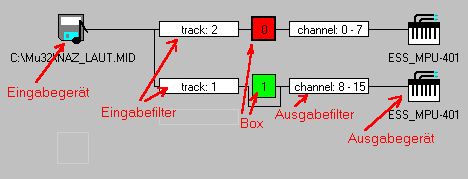
\includegraphics[width=234pt]{Route}
\fi
\end{center}

Über den Befehl "`\reflink{sec:MI_ROUTES}{Routes}"' im Menü
"`\reflink{sec:MS_VIEW}{View}"' kann das Fenster jederzeit in den
Vordergrund geholt werden.

Wie in der Abbildung sichtbar, werden die einzelnen Symbole im
Routenfenster bestimmten Funktionen zugeordnet. Diese Funktionen
\reflink{sec:eingabegerate}{Eingabegeräte},
\reflink{sec:eingabefilter}{Eingabefilter}, \ref{sec:boxen}{Boxen}, 
\ref{sec:ausgabefilter}{Ausgabefilter} und
\ref{sec:ausgabegerate}{Ausgabegeräte} sollen hier noch kurz
vorgestellt werden.

\helpsection{Route-Eingabegeraete}{MANUAL_ROUTE_INPUT_DEVICE}
\subsection{Eingabegeräte}\label{sec:eingabegerate}

Eingabegeräte entsprechen den Quellen, die Daten für \mutabor{} liefern 
sollen. Das können MIDI"=Geräte (Keyboards), MIDI"=Dateien 
oder GUIDO"=Dateien sein. Wenn Sie auf einem Gerät mit der Maus 
doppelklicken, öffnet sich ein entsprechender \reflink{sec:DE_R0}{Dialog},
in dem Sie das Gerät einstellen können (oder löschen).

Wenn ein Logikprogramm aktiviert ist, erscheinen neben den Icons 
für MIDI- oder GUIDO"=Dateien kleine Knöpfe, mit denen Sie 
das Abspielen der Dateien separat starten, stoppen, unterbrechen 
und fortsetzen können.

Um der Konfiguration ein neues Eingabegerät hinzuzufügen 
doppelklicken Sie mit der Maus im Routen"=Fenster in der Eingabegerätespalte 
zwischen zwei Eingabegeräte oder über dem ersten oder unter 
dem letzten, je nach dem, wo das neue Gerät eingefügt werden 
soll.


\helpsection{Route-Eingabefilter}{MANUAL_ROUTE_INPUT_FILTER}
\subsection{Eingabefilter}\label{sec:eingabefilter}

Eingabefilter ermöglichen es, die Datenströme nach verschiedenen Kriterien 
aufzuspalten und auch zu vervielfachen. So können Sie die entsprechenden 
Tondaten verschiedenen Umstimmungen und Ausgabegeräten zuordnen. 
Wenn sie auf einem Eingabefilter mit der linken Maustaste doppelklicken 
öffnet sich ein \reflink{sec:DE_R1}{Dialog}, in dem Sie die Einstellungen 
des Filters bearbeiten können. Beachten Sie, dass die möglichen 
Einstellungen auch von der Art des Eingabegerätes abhängen.


Mit einen Eingabefilter beginnen auch die eigentlichen Routen, 
die Verzweigungen. Wenn Sie einen Eingabefilter löschen, löschen 
Sie automatisch diesen Ast der Verzweigung.


Um einem Eingabegerät in der Konfiguration einen neue Eingabefilter 
(und somit eine neue Route) hinzuzufügen doppelklicken Sie 
mit der Maus im Routen"=Fenster in der Eingabefilterspalte zwischen 
zwei Filtern oder über dem ersten oder unter dem letzten, je 
nach dem, wo das neue Filter eingefügt werden soll.

\helpsection{Route-Boxen}{MANUAL_ROUTE_BOXES}
\subsection{Boxen}\label{sec:boxen}


Boxen sind abgeschlossene Einheiten, die die Umstimmautomatiken 
beinhalten und den Strom der musikalischen Daten mutieren (siehe 
mehr dazu im Abschnitt \tsciteref{sec:CO_BOX}). Wenn Sie mit 
der Maus auf einer Box doppelklicken (oder an der Stelle wo eigentlich 
eine sein sollte), öffnet sich ein \reflink{sec:DE_R2}{Dialog}, in dem 
Sie einstellen können, wie und welche Box in diesem Ast der 
Verzweigung arbeiten soll (jeder Datenstrom kann durch maximal 
eine Box geleitet werden).


\emph{Achtung:} In eine Box können aber mehrere Datenströme 
geleitet werden. In diesem Fall taucht die Box im Routen"=Fenster 
mehrfach auch. Es ist aber stets dieselbe Box gemeint. Beachten 
Sie auch, dass Sie in den Dialogen nicht Parameter der Box einstellen, 
sondern den Umgang Route mit der Box (und umgekehrt).


\emph{Wenn ein Logikprogramm aktiv ist}, könne Sie eine Box 
zur \reflink{sec:DV_CURRENTBOX}{aktuellen Box} machen indem Sie auf der 
entsprechenden Box doppelklicken. (diese reagiert dann z.\,B. auf 
die Buchstabentasten der Computer"=Tastatur).

\helpsection{Route-Ausgabefilter}{MANUAL_ROUTE_OUTPUT_FILTER}
\subsection{Ausgabefilter}\label{sec:ausgabefilter}

Ausgabefilter legen fest, welche MIDI"=Kanäle die Route zur Ausgabe der 
Töne verwenden darf, falls das Ausgabegerät ein MIDI"=Gerät 
oder eine MIDI"=Datei ist. Dies ist sinnvoll, wenn Sie bestimmte 
Kanäle vermeiden möchten oder nur bestimmte Kanäle verwenden 
möchten (weil Sie z.\,B. von Hand die Klangfarben einstellen). 
Um die Parameter einzustellen doppelklicken Sie mit der linken 
Maustaste auf dem Filter, es erscheint dann ein entsprechender 
\reflink{sec:DE_R3}{Dialog}.


\emph{Achtung:} Mutabor benötigt für jeden gleichzeitig erklingenden
Ton einen MIDI"=Kanal eigenen. Wählen Sie also möglichst einen großen
Bereich. Die Ausgabebereiche verschiedener Routen auf ein Gerät dürfen
sich ruhig überlappen. Eine interne Automatik verwaltet dann die
Kanäle und sorgt dafür, dass möglichst alle Töne erklingen und auch in
der gewünschten Klangfarbe. Stellen Sie also im Zweifelsfalle immer
0--15 ein.

\helpsection{Route-Ausgabegeraete}{MANUAL_ROUTE_OUTPUT_DEVICES}
\subsection{Ausgabegeräte}\label{sec:ausgabegerate}

Ausgabegeräte entsprechen den realen Ausgabegeräten und Tonerzeugern, die Sie
an den Computer angeschlossen haben. Wenn Sie mit der Maus auf einem
Ausgabegerät doppelklicken öffnet sich ein
\reflink{sec:DE_R4}{Dialog}, in dem Sie die Art und einzelne Parameter
des Gerätes einstellen können.


Es ist auch möglich, für eine Route überhaupt kein Ausgabegerät 
anzugeben (die Daten dieser Route werden dann auch nirgendwo ausgegeben). 
Dies ist im wesentlichen in zwei verschiedenen Szenarios sinnvoll:

\begin{itemize}
\item Wenn Sie bei einem Eingabegerät bestimmte Daten unterdrücken
  wollen (z.\,B. den Schlagzeug"=Track einer MIDI"=Datei). In diesem
  Fall würde weiter unten in der Konfiguration einen
  else"=Eingabefilter auftauchen der die restlichen Daten der
  gewünschten Box und Ausgabe zuleitet.
\item Wenn Sie die Daten dieser Route nur zum Ansteuern der
  Harmonieanalyse einer Box verwenden wollen. Diese Box kann dann
  wieder in anderen Routen zur Anwendung kommen. So können Sie z.B.
  bei einer MIDI"=Datei die Spur mit den Akkorden zum aktiven Steuern
  einer Box verwenden (ohne dass diese Akkorde erklingen), die dann
  passiv die Solostimme mutiert und ausgibt.
\end{itemize}


\helpsection{Logikfenster}{MANUAL_LOGIC_WINDOW}
\section{Logiken"=Fenster}\label{sec:DE_LOGIC}
In diesem Fenster sehen Sie für eine Box die Logiken und Umstimmungen,
die sie mit der Computertastatur auslösen können. Logiken sind als
Ordner dargestellt, einfache Umstimmungen als weiße Blätter. Die
aktuelle Logik ist ein geöffneter Ordner, die aktuelle Umstimmung
erhält eine Note auf dem Blatt. In jedem Symbol erscheint der
Buchstabe, der diese Aktion auslöst. Man kann aber auch den Cursor mit
den Pfeiltasten bewegen und mit der Enter"=Taste die gerade gewählt
Logik/""Umstimmung aktivieren.  Dies ist auch durch Doppelklick der Maus
möglich. In der Regel ändert sich der Inhalt dieses Fensters
entsprechend der ausgelösten Aktionen.


Sobald Sie dieses Fenster durch einen Mausklick in den Vordergrund
holen wird die zugeordnete \reflink{sec:DV_BOX}{Box} zur
\reflink{sec:DV_CURRENTBOX}{aktuellen Box} und reagiert dann auf
Buchstabentasten.


Wenn Sie alle Logiken"=Fenster schließen, wird die Ausführung des
aktuellen \mutabor{}"=Programms abgebrochen wie bei einem
\reflink{sec:MI_STOP}{Stop"=Befehl}.


Wenn ein \reflink{sec:DV_LOGIKPROGRAMM}{Logikprogramm}
\reflink{sec:MI_ACTIVATE}{aktiviert} ist, erhalten Sie durch Klicken
mit der rechten Maustaste ein kleines Popup"=Menü, in dem Sie
einstellen können, welche \reflink{sec:DV_BOX}{Box} als
\reflink{sec:DV_CURRENTBOX}{aktuelle Box} fungieren soll und welche
\reflink{sec:DV_PROTOKOLL}{Protokollfenster} angezeigt werden sollen.

\helpsection{Fenster-Aktuelle-Tasten}{MANUAL_CURRENT_KEYS_WINDOW}
\section{Aktuelle"=Tasten"=Fenster}\label{sec:DE_KEY}
In diesem Fenster wird angezeigt, welche Töne gerade in den
Datenströmen der entsprechenden Box anliegen, es handelt sich somit um
die "`liegenden Töne"' in einer Box (die dann auch für die
Harmonieanalyse interessant sind). Dies sind z.\,B. meist die
Klaviatur"=Tasten, die auf dem Steuer"=Keyboard gerade gedrückt sind.
Die Anzeige erfolgt als \reflink{sec:DV_MIDI}{MIDI"=Nummern} der
Tasten.


Ob das Fenster angezeigt wird, kann im Menü
"`\reflink{sec:MS_VIEW}{View}"' im Punkt
"`\reflink{sec:MI_KEY}{Current Keys}"' ausgewählt werden.

Sobald Sie dieses Fenster durch einen Mausklick in den Vordergrund
holen wird die zugeordnete \reflink{sec:DV_BOX}{Box} zur
\reflink{sec:DV_CURRENTBOX}{aktuellen Box} und reagiert dann auf
Buchstabentasten.


Wenn ein \reflink{sec:DV_LOGIKPROGRAMM}{Logikprogramm}
\reflink{sec:MI_ACTIVATE}{aktiviert} ist, erhalten Sie durch Klicken
mit der rechten Maustaste ein kleines Popup"=Menü, in dem Sie
einstellen können, welche \reflink{sec:DV_BOX}{Box} als
\reflink{sec:DV_CURRENTBOX}{aktuelle Box} fungieren soll und welche
\reflink{sec:DV_PROTOKOLL}{Protokollfenster} angezeigt werden sollen.


Wenn der \reflink{sec:DV_OWM}{Ein"=Fenster"=Modus} aktiv ist, gibt es immer 
nur ein Aktuelle"=Tasten"=Fenster, das die liegenden Töne der 
jeweils \reflink{sec:DV_CURRENTBOX}{aktuellen Box} anzeigt.


\helpsection{Tonsystemfenster}{MANUAL_WINDOW_TONE_SYSTEM}
\section{Tonsystem"=Fenster}\label{sec:DE_TS}
In diesem Fenster wird angezeigt, mit welchem Tonsystem die
entsprechende Box gerade arbeitet, d.\,h. in welchem Stadium sich die
Logiken gerade befinden. Es dazu werden die einzelnen Töne des Systems
mit den entsprechenden Sequenzen angegeben.


Ob das Fenster angezeigt wird, kann im Menü \reflink{sec:MS_VIEW}{View} 
im Punkt \reflink{sec:MI_TS}{Tone system} ausgewählt werden.


Sobald Sie dieses Fenster durch einen Mausklick in den Vordergrund
holen wird die zugeordnete \reflink{sec:DV_BOX}{Box} zur
\reflink{sec:DV_CURRENTBOX}{aktuellen Box} und reagiert dann auf
Buchstabentasten.


Wenn ein \reflink{sec:DV_LOGIKPROGRAMM}{Logikprogramm}
\reflink{sec:MI_ACTIVATE}{aktiviert} ist, erhalten Sie durch Klicken
mit der rechten Maustaste ein kleines Popup"=Menü, in dem Sie
einstellen können, welche \reflink{sec:DV_BOX}{Box} als
\reflink{sec:DV_CURRENTBOX}{aktuelle Box} fungieren soll und welche
\reflink{sec:DV_PROTOKOLL}{Protokollfenster} angezeigt werden sollen.


Wenn der \reflink{sec:DV_OWM}{Ein"=Fenster"=Modus} aktiv ist, gibt es
immer nur ein Tonsystem"=Tasten"=Fenster, dass das Tonsystem der
jeweils \reflink{sec:DV_CURRENTBOX}{aktuellen Box} anzeigt.




\helpsection{Aktionsfenster}{MANUAL_ACTIONS_WINDOW}
\section{Aktionen"=Fenster}\label{sec:DE_ACTION}
In diesem Fenster wird angezeigt, welche Aktionen die zugeordnete 
Box seit \reflink{sec:MI_ACTIVATE}{Start des Logikprogramms} durchgeführt 
hat. Es werden dazu die im Programmtext verwendeten Namen der 
entsprechenden Umstimmungen angegeben.


Ob das Fenster angezeigt wird, kann im Menü \reflink{sec:MS_VIEW}{View} 
im Punkt \reflink{sec:MI_ACTION}{Actions} ausgewählt werden.


Sobald Sie dieses Fenster durch einen Mausklick in den Vordergrund
holen wird die zugeordnete \reflink{sec:DV_BOX}{Box} zur
\reflink{sec:DV_CURRENTBOX}{aktuellen Box} und reagiert dann auf
Buchstabentasten.


Wenn der \reflink{sec:DV_OWM}{Ein"=Fenster"=Modus} aktiv ist, gibt es
immer nur ein Aktionen"=Fenster, dass die Umstimmungen der jeweils
\reflink{sec:DV_CURRENTBOX}{aktuellen Box} anzeigt. Wenn der
\reflink{sec:DV_CAW}{Gemeinsames"=Aktionen"=Fenster"=Modus} aktiv ist,
werden die Aktionen \emph{aller}
\reflink{sec:DV_BOX}{Boxen} in \emph{einem} Fenster
angezeigt (den Umstimmungen wird dann jeweils die Nummer der Box
vorangestellt).


Wenn ein \reflink{sec:DV_LOGIKPROGRAMM}{Logikprogramm}
\reflink{sec:MI_ACTIVATE}{aktiviert} ist, erhalten Sie durch Klicken
mit der rechten Maustaste ein kleines Popup"=Menü, in dem Sie
einstellen können, welche \reflink{sec:DV_BOX}{Box} als
\reflink{sec:DV_CURRENTBOX}{aktuelle Box} fungieren soll und welche
\reflink{sec:DV_PROTOKOLL}{Protokollfenster} angezeigt werden sollen.



\helpsection{Compilerfenster}{MANUAL_WINDOW_COMPILER}
\section{Compiler"=Fenster}\label{sec:DE_COMP}
Dieses Fenster ist nur während und nach der Programmübersetzung 
zu sehen.

Es werden die gerade übersetzte Datei, die Anzahl der Zeilen, 
die Anzahl verschiedener \mutabor{}"=Konstrukte und evtl. Fehlermeldungen 
angezeigt.

Mit Hilfe des breiten Knopfes im unteren Fensterbereich lässt 
sich das Fenster schließen.

\helpsection{Hilfefenster}{MANUAL_HELP_WINDOW}
\chapter{Das Hilfefenster}\label{sec:HELPWINDOW}

Die verschiedenen Hilfe-Menüpunkte und Hilfe-Knöpfe öffnen das
Hilfefenster. An der rechten Seite finden Sie gelegentlich eine
Bildlaufleiste, an der Sie die Hilfeseite mit Hilfe der Maus auf eine
geeignete Position führen können. Die Seite können Sie auch mit Hilfe
der Tasten \LArrow, \UArrow, \DArrow, \RArrow, \PgUp{} und \PgDown{}
verschieben.

Weiterhin gibt es Verknüpfungen. Ein Klick mit der Maus darauf öffnet die 
zugehörige Seite im Hilfefenster. 

Beispiel: \reflink{sec:HELPWINDOW}{Verknüpfung auf diese Seite}.

\ifhtml
\HCode{<img src=\dq Hilfefenster.png\dq align=\dq right\dq />}
\else
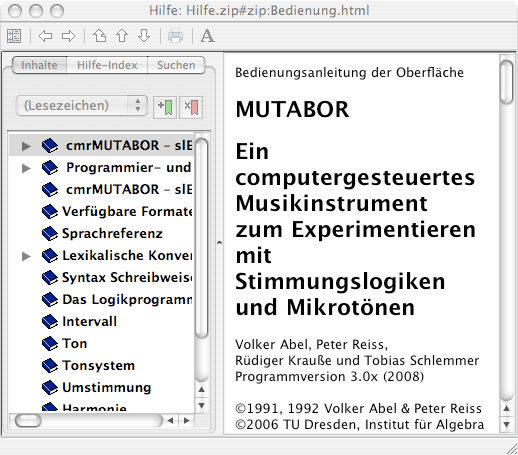
\includegraphics{Hilfefenster}
\fi

Die folgenden Abschnitte beschreiben die einzelnen Bereiche des Hilfefensters:

\helpsection{Hilfe-Symbolleiste}{MANUAL_HELP_TOOLBAR}
\section{Die Symbolleiste}
\label{sec:die-symbolleiste}

\ifhtml
\Picture[Symbolleiste]{{helptoolbar.png} align=\dq left\dq}%
\else

\includegraphics{helptoolbar}
\fi

Am oberen Fensterrand befindet sich die Symbolleiste. Die einzelnen Symbole können mit der Maus angeklickt werden. Dabei können Sie folgendes machen:

\begin{description}
\item[\mutimage{{htmsidep.png}}{{htmsidep}}~Suchbaum ein-/ausschalten] Mit diesem Symbol kann links das Suchbaum-Fenster ein- bzw. ausgeschaltet werden. So kann ggf. mehr Platz für den Hilfetext geschaffen werden.
\item[\mutimage{{back}}{{back}}~letzte HTML-Seite anzeigen] Mit diesem Symbol kann man zu der Seite zurückspringen, die vor der aktuellen angesehen wurde.
\item[\mutimage{{forward}}{{forward}}~nächste HTML-Seite anzeigen] Mit diesem Symbol kann man in der Geschichte eine Seite vorspringen, wenn man sich nach der aktuellen Seite schon einmal eine andere angesehen hatte und zurückgesprungen war.
\item[\mutimage{{toparent}}{{toparent}}~In die nächste Dokumenteben gehen] Hier kann man eine Kapitelebene nach oben gehen.
\item[\mutimage{{up}}{{up}}~Vorherige Seite]~Hier kann man zum vorhergehenden Abschnitt im entsprechenden Handbuch wechseln.
\item[\mutimage{{down}}{{down}}~Nächste Seite]~Hier kann man zum folgenden Abschnitt im entsprechenden Handbuch wechseln.
\item[\mutimage{{print}}{{print}}~Diese Seite Drucken]~Mit diesem Werkzeug können sie die aktuell angezeigte Seite ausdrucken.
\item[\mutimage{{htmoptns}}{{htmoptns}}~Einstellungen-Dialog]~Hier können Sie die Einstellungen (Schrift usw.) von Ihrem Hilfefenster beeinflussen. 
\end{description}

\helpsection{Hilfe-Navigationsfenster}{MANUAL_HELP_NAVIGATION}
\section{Das Navigationsfenster}
\label{sec:der-suchbaum}

\mutimage{{Hilfeinhaltsbaum}}{{Hilfeinhaltsbaum}}

Das Navigationsfenster besitzt drei Reiter:
\begin{itemize}
\item Den Dokumentbaum („Inhalte“),
\item den Hilfeindex („Hilfe-Index“) und
\item das Suchformular („Suchen“).
\end{itemize}

Klicken Sie auf den gewünschten Reiter, um sich die entsprechenden
Bedienelemente anzeigen zu lassen!

\helpsection{Dokumentbaum}{MANUAL_DOCUMENT_TREE}
\subsection{Der Dokumentbaum}
\mutimage{{Hilfeinhaltsbaum}}{{Hilfeinhaltsbaum}}

Der Dokumentbaum dient dafür, einzelne Kapitel schnell anspringen zu
können. Dabei werden die Unterkapiteln den jeweils übergeordneten
zugeordnet. Ein Buch (\mutimage{{htmbook}}{{htmbook}}) oder Ordner
(\mutimage{{htmfoldr}}{{htmfoldr}}) kann aufgeklappt werden, um die darin
enthaltenen Abschnitte angzeigt zu bekommen. Dazu genügt es mit der
linken Maustaste auf die entsprechende Zeile zu klicken. Einzelne
Seiten werden durch ein Blatt Papier
(\mutimage{{htmpage}}{{htmpage}}) symbolisiert. Auch sie können
angeklickt werden.

Oberhalb des Baumes können Sie Lesezeichen anlegen. Möchten Sie ein
Lesezeichen hinzufügen, klicken Sie dazu einfach auf das zugehörige
Symbol mit einem kleinen „+“
(\mutimage{{addbookm}}{{addbookm}}). Danach können Sie die Seite
jederzeit in der Auswahl links neben dem Knopf aktivieren. Ein Klick
auf den Knopf mit dem kleinen „x“ (\mutimage{{delbookm}}{{delbookm}})
entfernt das Lesezeichen wieder.

\helpsection{Hilfeindex}{MANUAL_HELP_INDEX}
\subsection{Der Hilfeindex}
\mutimage{{Hilfeindex}}{{Hilfeindex}}

Die Hilfe enthält ähnlich einem guten Handbuch ein
Stichwortverzeichnis bzw. Index. Wenn Sie ein Wort suchen ist der Index zunächst einmal die richtige Anlaufstelle. Geben Sie das Wort oben in das Eingabefeld ein und drücken Sie auf „Suchen“! Es erscheint gleich darauf eine Auswahl von Stichworten, die zu Ihrer Suchanfrage passen. Alternativ können sie sich auch alle Stichworte mit dem Knopf „Alles zeigen“ anzeigen lassen.

\helpsection{Suchformular}{MANUAL_SEARCH_FORM}
\subsection{Das Suchformular}
\mutimage{{Hilfesuchformular}}{{Hilfesuchformular}}

Wenn der Index nicht ausreicht, gibt es auch die Möglichkeit, das
gesamte Dokument zu durchsuchen. Geben Sie im Eingabefeld das
gewünschte Suchwort ein! Darunter können Sie auswählen, in welchen
Handbüchern gesucht werden soll. Markieren Sie
„Groß-/Kleinschreibung“, wenn sie Groß- von Kleinbuchstaben
unterscheiden wollen und „Nur ganze Wörter“, wenn Sie nur eigene
Wörter, aber keine Wortteile finden möchten. Klicken Sie nun auf
„Suchen“ und es werden Ihnen unterhalb des Knopfes die gefundenen
Textstellen angezeigt. Diese können Sie anklicken und damit im
nebenstehenden \reflink{sec:das-textfenster}{Textfenster} anzeigen
lassen.

\helpsection{Hile-Textfenster}{MANUAL_HELP_TEXT}
\section{Das Textfenster}
\label{sec:das-textfenster}

\mutimage{{Hilfetextfenster}}{{Hilfetextfenster}}

Im Textfenster wird der eigentliche Hifetext angezeigt. Die wesentliche Bedienung wurde schon im Abschnitt \nameref{sec:HELPWINDOW} beschrieben und soll hier nicht wiederholt werden.

\helpsection{Dialoge}{MANUAL_DIALOGS}
\chapter{Dialoge}\label{sec:DE_DIALOGS}

In diesem Kapitel sollen die Dialoge von \mutabor{} kurz vorgestellt
werden.  Dialoge sind Fenster, die im Vordergrund aufgehen, wenn Sie
oder \mutabor{} bestimmte Aktionen ausführen. Im Gegensatz zu den
\reflink{sec:DE_SUBWINDOW}{Unterfenstern} befinden sie sich nicht
innerhalb des Hauptfensters.

Solange ein Dialog offen ist, sind alle anderen \mutabor"=Fenster
gesperrt. Sie können dort also keine Eingaben machen und auch keine
Aktionen ausführen. Erst wenn der Dialog geschlossen ist, werden die
anderen Fenster wieder freigegeben.

Dialoge dienen dazu, um Eingaben zu machen und Informationen
anzuzeigen, die Sie bestätigen sollen.  

\helpsection{Eingabegeraetedialog}{HELP_INPUT_DEVICE_DIALOG}
\section{Eingabegeräte"=Dialog}
\label{sec:DE_R0}
Dieser Dialog lässt sich für die Eingabegeräte vom \reflink{sec:DE_ROUTES}{Routen"=Fenster} 
aus aufrufen, indem Sie auf einem Eingabegerät mit der Maus 
Doppelklicken. In ihm wird das Gerät bzw. die Datei spezifiziert.

\helpsection{Eingabegeraetetyp}{MANUAL_INPUT_DEVICE_TYPE}
\subsection{Type (Typ des Eingabegerätes)}


Hier geben Sie den Grundtyp des Gerätes an. Es gibt drei mögliche 
Einstellungen, die anderen Eingaben des Dialogs passen sich dementsprechend 
an.

\begin{description}
\item[Type: MIDI device] (\reflink{sec:DV_MIDI}{MIDI}"=Gerät)
  Wählen Sie diese Option, wenn das Gerät ein normales MIDI"=Gerät
  sein soll (z.\,B. Keyboard). Wählen Sie dann in der Liste "`Device
  name"' den \reflink{sec:DV_PORT}{MIDI"=Port} aus, an den dieses
  Gerät angeschlossen ist.

\item[Type: MIDI file] (\reflink{sec:DV_MIDIFILE}{MIDI"=Datei})
  In diesem Fall soll das Gerät eine
  \reflink{sec:DV_MIDIFILE}{MIDI"=Datei} sein, die dann abgespielt
  werden kann. Geben Sie unter MIDI file name den Namen der
  entsprechenden Datei ein. Mit Durchsuchen können Sie auch den
  üblichen Dateien"=Dialog öffnen und so die Datei angeben.

\item[Type: GUIDO file] (\reflink{sec:DV_GUIDO}{GUIDO"=Datei}) Hiermit
  geben Sie an, dass zur Eingabe eine GUIDO"=Datei verwendet werden
  soll. Geben Sie dazu unter GUIDO file name den Namen der gewünschten
  Datei ein. Mit Durchsuchen können Sie auch den üblichen
  Dateien"=Dialog öffnen und so die Datei angeben.
\end{description}


Mit "`OK"' können Sie ihre Eingaben bestätigen oder den Dialog mit Abbruch
beenden ohne gemachte Änderungen zu übernehmen.  Mit "`Löschen"'
können Sie das Gerät samt der zugeordneten Routen aus der
Konfiguration entfernen.

\helpsection{Eingabefilterdialog}{MANUAL_INPUT_FILTER_DIALOG}
\section{Eingabefilter"=Dialog}\label{sec:DE_R1}
Dieser Dialog lässt sich für die Routen vom
\reflink{sec:DE_ROUTES}{Routen"=Fenster} aus aufrufen, indem Sie auf
einem Eingabefilter mit der Maus Doppelklicken. In ihm werden die
Einstellungen des Filters spezifiziert.

\helpsection{Eingabefiltertyp}{MANUAL_INPUT_FILTER_TYPE}
\subsection{Type (Type des Filters)}

\begin{description}
\item[all:] (alles) In diesem Modus lässt der Filter alle Daten
  passieren.
\item[else:] (ansonsten, Restliche Daten) Dieser Filter lässt alle
  Daten des Eingabegerätes durch, die nicht schon in einer anderen
  Route vom entsprechenden Filter durchgelassen wurden. Dies bezieht
  sich auf die Routen, die oberhalb der else"=Route angeordnet sind.
  Praktischer Weise findet man solche Filter meist in der letzten
  Route.
\item[chanel:] (Kanal, nur bei \reflink{sec:DV_MIDI}{MIDI}"=Geräten und
  \reflink{sec:DV_MIDIFILE}{MIDI"=Dateien}) Hier werden nur die Daten
  durchgelassen, deren MIDI"=Kanalnummern innerhalb der in Range
  eingestellten Werte liegen. Meist liegen Stimmen mit verschiedenen
  Klangfarben auf verschiedenen Kanälen, auf diese Weise können Sie
  MIDI"=Dateien bequem aufspalten.

  Beachten Sie bitte, dass \mutabor{} die Zählung mit 0 beginnt, d.\,h.
  es gibt die Kanäle 0 bis 15.

\item[key range:] (Ton"=Umfang, nur bei MIDI"=Geräten) Diese Option
  ist ein Behelf für Keybords, um deren Tastatur in mehrere Sektionen
  aufzuteilen. Dieser Filter lässt nur Tondaten durch, deren
  \reflink{sec:DV_MIDINOTES}{MIDI"=Nummer der Taste} innerhalb der in
  Range eingestellten Werte liegt. So können Sie die Klaviatur in
  beliebig viele Bereiche aufsplitten, die sie auch überschneiden
  dürfen. In der Regel bieten Keyboards aber von sich aus die
  Möglichkeit einer solchen Splittung (allerdings meist ohne
  Überlappung) und ordnet die Sektionen verschiedenen MIDI"=Kanälen zu.
  Dies ist auch die allgemein zu empfehlende Variante (wenn dies
  möglich ist).

\item[track:] (Ton"=Spur, nur bei MIDI"=Dateien) Die Daten in
  MIDI"=Dateien sind in der Regel in mehrere Tracks gegliedert. Bei
  dieser Einstellung lässt der Filter nur die Daten der Tracks durch,
  deren Nummern innerhalb der in Range eingestellten Werte liegen.


\item[box tag:] (Boxen"=Tag, nur bei
  \reflink{sec:DV_GUIDO}{GUIDO"=Dateien}) In dieser Einstellung lässt
  der Filter bei GUIDO"=Dateien nur die Daten durch, deren mit dem
  Box"=Tag zugeordnete Nummern innerhalb der in Range eingestellten
  Werte liegen.


\item[staff:] (Notensystem, nur bei GUIDO"=Dateien) In diesem Fall
  werden die Daten der Notensysteme durchgelassen, deren Nummern
  innerhalb der in Range eingestellten Werte liegen. Die Nummerierung
  beginnt bei 1.
\end{description}


\helpsection{Eingabefilterbereich}{MANUAL_INPUT_FILTER_RANGE}
\subsection{Bereich:}

Bestimmt einen Wertebereich, der je nach Typ des Filters interpretiert
wird. Die eingestellten Randwerte zählen mit zum Wertebereich.

Mit "`OK"' können Sie ihre Eingaben bestätigen oder den Dialog mit Abbruch
beenden ohne gemachte Änderungen zu übernehmen.  Mit "`Löschen"'
können Sie die Route aus der Konfiguration entfernen.


Um eine neue Route anzulegen doppelklicken Sie im
\reflink{sec:DE_ROUTES}{Routen"=Fenster} in der Eingabefilter"=Spalte
zwischen die zwei Filter, zwischen denen die neue Route eingefügt
werden soll, bzw. oberhalb der ersten Route oder unterhalb der
letzten, wenn die Route dort angelegt werden soll.

Sie können einem Eingabegerät mehrere Eingabefilter zuordnen. 
Auf diese Weise können Sie de Datenstrom im mehrere Routen 
aufspalten. Die Vielzahl der Typen der Eingabefilter erlaubt 
ihnen einen flexiblen Umgang mit den Daten.

\helpsection{Eingabefilter-Hinweis}{MANUAL_INPUT_FILTER_ADVISE}
\subsection{Tipp/""Hinweis:}
Was tun, wenn z.\,B. die Daten der MIDI"=Kanäle 1 und 3 in eine 
spezielle Box weitergeleitet werden sollen?

Wenn man bei Range 1--3 eingeben würde, würden auch die 
Daten von Kanal 2 mit durchgelassen werden, was ja nicht beabsichtigt 
ist. Legen Sie in diesem Fall \emph{zwei} Routen mit Kanal"=Filtern 
an, geben Sie bei Range 1--1 und 3--3 an und leiten Sie beide 
Routen in dieselbe gewünschte Box. 

\helpsection{Boxendialog}{MANUAL_BOX_DIALOG}
\section{Boxen"=Dialog}\label{sec:DE_R2}

Dieser Dialog lässt sich für die Routen vom \reflink{sec:DE_ROUTES}{Routen"=Fenster} 
aus aufrufen, indem Sie auf einer Box mit der Maus Doppelklicken. 
In ihm werden die Einstellungen dieser Box spezifiziert.

\helpsection{Boxtyp}{MANUAL_BOX_TYPE}
\subsection{Box (Art der Box)} Wählen Sie hier dir gewünschte Art der
Box aus.

\begin{description}
\item[box nummer (Box mit Nummer, Standardfall)] Bei dieser Variante
  geben Sie der Box eine Nummer (zwischen 0 und 255). über diese
  Nummer ist die Box ansprechbar, erhält bei gestartetem Logikprogramm
  ein Logiken"=Fenster und kann über die Protokoll"=Fenster überwacht
  werden. Zur bequemeren Unterscheidung werden im Routen"=Fenster
  verschiedenen Boxen durch verschiedene Farben dargestellt
\item[GUIDO"=File (Reaktion auf Tags aus GUIDO"=Datei)] Diese Variante
  kann verwendet, werden, wenn das Eingabegerät eine GUIDO"=Datei ist.
  In diesem Fall erhält die Box keine spezielle Nummer und reagiert
  auf Steuer"=Tags der GUIDO"=Datei.
\item[no box / thru mode (Keine Box, Durchgangsmodus)] In diesem Fall
  schaltet die Route auf ``Durchgang'', die Daten werden durch keine
  Box geleitet, sondern direkt zum Ausgabegerät.  Im Routen"=Fenster
  wird dann an dieser Stelle auch keine Box dargestellt.
\end{description}

\helpsection{Boxmodus}{MANUAL_BOX_MODE}
\subsection{Mode (Modus der Box)}
\begin{description}
\item[active (Aktiver Modus, Steuer"=Modus)] Beim aktivem Modus werden
  die eingehenden Daten auf Steuerinformationen geprüft und der
  Harmonieanalyse zugeführt und anschließend mutiert weitergegeben.
  Die Daten werden also zur Steuerung der Box herangezogen.

  Im Routen"=Fenster werden diese Boxen mit dickem Rahmen dargestellt.
\item[passiv (Passiver Modus)] Im passiven Modus werden die Daten
  nicht zur Steuerung herangezogen sondern nur entsprechend des
  aktuellen Tonsystems der Box mutiert und weitergeleitet. Die Daten
  können den Zustand der Box nicht beeinflussen.


  Im Routen"=Fenster werden diese Boxen mit dünnem Rahmen dargestellt.
\end{description}


Mit "`OK"' können Sie ihre Eingaben bestätigen oder den Dialog 
mit "`Abbruch"' beenden ohne gemachte Änderungen zu übernehmen.

Wenn eine Box im Routen"=Fenster mehrfach auftaucht, so ist trotzdem
stets dieselbe Box gemeint. Es ist dann egal, auf welcher Box Sie
doppelklicken um diesen Dialog zu öffnen, er enthält stets die
gleichen Daten.

\helpsection{Ausgabefilterdialog}{MANUAL_OUTPUT_FILTER_DIALOG}
\section{Ausgabefilter"=Dialog}\label{sec:DE_R3}
Dieser Dialog lässt sich für die Routen vom \reflink{sec:DE_ROUTES}{Routen"=Fenster} 
aus aufrufen, indem Sie auf einem Ausgabefilter mit der Maus 
Doppelklicken. In ihm werden die Einstellungen des Filters spezifiziert. 
Die Ausgabefilter gibt es nur, wenn das Ausgabegerät ein MIDI"=Gerät 
oder eine MIDI"=Datei ist.

\helpsection{Ausgabefilter-MIDI-Kanaele}{MANUAL_OUTPUT_FILTER_MIDI_CHANNELS}
\subsection{Channel (MIDI"=Kanäle)}
Geben Sie an, welche MIDI"=Kanäle auf dem Ausgabegerät verwendet 
werden dürfen. Achten Sie darauf, dass bei \mutabor{} die 
Kanalzählung bei 0 beginnt, Sie können also maximal 0--15 
angeben.

Je mehr Kanäle sie angeben, um so weniger Probleme gibt es bei der
Klangausgabe von Akkorden (Da Mutabor für jeden klingenden Ton einen
Kanal benötigt, können z.\,B. bei einer Einstellung von 0"=7 nur maximal
8 Töne gleichzeitig erklingen. Bei einer Raschen Tonfolge mit einer
nachhallenden Klangfarbe können bei knapp bemessener Kanalzahl
"`Jaul"'"=Effekte auftreten.)

Die Kanäle verschiedener Routen, die das gleiche Ausgabegerät 
verwenden dürfen sich auch überschneiden. Dies ist zu empfehlen, 
wenn Sie nicht von außerhalb die Klangfarben der Kanäle andern 
müssen, das so den einzelnen Routen u.\,U.\ mehr Kanäle zur 
Verfügung stehen. Eine interne Automatik verteilt dann jeweils 
die Kanäle nach aktuellem Bedarf, wobei Sie natürlich auch 
die aktuellen Klangfarben berücksichtigt.

Mit "`OK"' können Sie ihre Eingaben bestätigen oder den Dialog 
mit Abbruch beenden ohne gemachte Änderungen zu übernehmen.

\helpsection{Ausgabegeraetedialog}{MANUAL_OUTPUT_DEVICE_DIALOG}
\section{Ausgabegerät"=Dialog}
\label{sec:DE_R4}

Dieser Dialog lässt sich für die Ausgabegeräte vom \reflink{sec:DE_ROUTES}{Routen"=Fenster} 
aus aufrufen, indem Sie auf einem Ausgabegerät mit der Maus 
Doppelklicken. In ihm wird das Gerät bzw. die Datei spezifiziert.

\helpsection{Ausgabetyp}{MANUAL_OUTPUT_DEVICE_TYPE}
\subsection{Type (Typ des Ausgabegerätes)}

Hier geben Sie den Grundtyp des Gerätes an. Es gibt drei mögliche 
Einstellungen, die anderen Eingaben des Dialogs passen sich dementsprechend 
an.

\begin{description}
\item[Type: MIDI device (\reflink{sec:DV_MIDI}{MIDI}"=Gerät)] Wählen
  Sie diese Option, wenn das Gerät ein normales MIDI"=Gerät sein soll
  (z.\,B. Synthesizer, Keyboard, Expander). Wählen Sie dann in der Liste
  Device name den \reflink{sec:DV_PORT}{MIDI"=Port} aus, an den dieses
  Gerät angeschlossen ist.

  Bei "`Bending range"' müssen die \reflink{sec:DV_BENDINGRANGE}{Bending
    range} angeben, die auf diesem Gerät eingestellt ist.

\item[Type: MIDI file (\reflink{sec:DV_MIDIFILE}{MIDI"=Datei})] In
  diesem Fall werden die Daten in einer
  \reflink{sec:DV_MIDIFILE}{MIDI"=Datei} abgelegt. Geben Sie unter
  MIDI file name einen Namen für diese Datei an. Mit Durchsuchen
  können Sie auch den üblichen Dateien"=Dialog öffnen und so die Datei
  angeben.

  Bei "`Bending range"' müssen Sie die
  \reflink{sec:DV_BENDINGRANGE}{Bending range} angeben, die beim
  Abspeichern verwendet werden soll.

\item[Type: GUIDO file (\reflink{sec:DV_GUIDO}{GUIDO"=Datei})] Hiermit
  geben Sie an, dass die Musikdaten in eine GUIDO"=Datei geleitet
  werden sollen. Geben Sie dazu unter GUIDO file name einen Namen für
  die gewünschte Datei ein. Mit Durchsuchen können Sie auch den
  üblichen Dateien"=Dialog öffnen und so die Datei angeben.
\end{description}

Mit "`OK"' können Sie ihre Eingaben bestätigen oder den Dialog 
mit "`Abbruch"' beenden ohne gemachte Änderungen zu übernehmen. 
Mit "`Löschen"' können Sie das Gerät aus der Konfiguration 
entfernen; die Daten dieser Route werden dann nirgendwo ausgegeben, 
können aber evtl. zum Steuern einer \reflink{sec:DV_BOX}{Box} verwendet 
werden.

Wenn ein Ausgabegerät im Routen"=Fenster mehrmals auftaucht, 
ist trotzdem stets dasselbe Gerät gemeint. Es ist dann egal, 
auf welches Gerät Sie klicken, es öffnet sich stets der selbe 
Dialog.

\helpsection{Ueber-Fenster}{MANUAL_ABOUT_WINDOW}
\section{Über…"=Fenster}\label{sec:DE_ABOUT}

Dieses Fenster zeigt lediglich, das Sie tatsächlich mit \mutabor{} 
arbeiten und enthält kurze Informationen zum Programm und zur 
Version.

\helpsection{Eintstellungsdialog}{MANUAL_SETTINGS_DIALOG}
\section{Der Einstellungsdialog}\label{sec:DE_SETUP}
Hier können Sie einige globale Parameter von \mutabor{} einstellen.

\helpsection{Einstellungen-Tonsystem}{MANUAL_SETTINGS_TONE_SYSTEM}
\subsection{Tonsytem}
Ansicht der Tonsysteme im
\reflink{sec:DE_KEY}{Aktuelle"=Tasten"=Fenster} und
\reflink{sec:DE_TS}{Tonsystem"=Fenster}.
\begin{description}
\item[als Relationen:] Bei dieser Einstellung werden
  die einzelnen Töne als \reflink{sec:DV_CENT}{Cent}"=Abstände zum
  \reflink{sec:DV_BASETONE}{Verankerungston} angegeben)
\item[als Tonsystem:] Die einzelnen Töne werden als
  absolute Frequenzen und \reflink{sec:DV_MIDINOTES}{MIDI"=Noten}
  angegeben.
\end{description}

\helpsection{Einstellungen-Fenster}{MANUAL_SETTINGS_WINDOWS}
\subsection{Fenster}
\begin{description}
\item[Speichere Editor-Dateien:] ist diese Option
  eingeschaltet, so wird der \reflink{sec:DV_QUELLTEXT}{Quelltext} in
  den \reflink{sec:DE_EDIT}{Editorfenstern} gespeichert, bevor ein
  \reflink{sec:DV_LOGIKPROGRAMM}{Logikprogramms} aktiviert wird.  Das
  kann sinnvoll sein, wenn Sie mit instabilen
  \reflink{sec:DV_MIDI}{MIDI"=Konfigurationen} experimentieren.
\item[Nutze Farbbalken:] Jeder
  \reflink{sec:DV_BOX}{Box} ist in \mutabor{} eine Farbe zugeordnet.
  ist diese Option aktiviert, so erscheinen in den
  \reflink{sec:DE_LOGIC}{Logik-} und
  \reflink{sec:DV_PROTOKOLL}{Protokollfenstern} die Farben der
  zugehörigen Boxen. Dies ist sehr zu empfehlen, wenn man mit
  verschiedenen Boxen gleichzeitig arbeitet.
\end{description}

Mit OK können Sie ihre Eingaben bestätigen oder den Dialog 
mit Abbruch beenden ohne gemachte Änderungen zu übernehmen.




\helpsection{Sprachgrundlagen}{MANUAL_LANGUAGE_BASICS}
\part{Grundlagen der \mutabor sprache}
\label{sec:SX_BASICS}

\helpsection{Grundlegendes}{MANUAL_BASICS}
\chapter{Grundlegendes}

\mutabor{} arbeitet mit
\reflink{sec:DV_LOGIKPROGRAMM}{Logikprogrammen}. Das sind Texte in der
\mutabor{}"=Programmiersprache, die
\reflink{sec:MI_COMPILE}{übersetzt} und
\reflink{sec:MI_ACTIVATE}{aktiviert} werden. Diese
\reflink{sec:DV_QUELLTEXT}{Quelltexte} können in den
\reflink{sec:DE_EDIT}{Editor"=Fenstern} geschrieben werden.

Die \mutabor{}sprache arbeitet ereignisgesteuert: Ein
\mutabor{}programm besteht aus Anweisungen, die angeben, wie auf
bestimmte Ereignisse reagiert werden soll. Ereignisse sind dabei
Eingaben über die Tastatur, aktuell auf Eingabegerät (MIDI"=Datei oder
Keyboard) gespielte Tonmuster oder zusätzliche in der MIDI"=Datei
eingetragene Informationen. Reaktionen sind Umstimmungsbefehle.

Somit hat ein \mutabor{}"=Programm die folgenden Teile:

\begin{itemize}
\item Definition der \reflink{sec:SX_TONE}{Töne}, aus denen sich die
  Tonleitern zusammensetzen sollen; dies geschieht mit Hilfe der
  ebenfalls zu definierenden \reflink{sec:SX_INTERVAL}{Intervalle}.
\item Definition der \reflink{sec:SX_TONESYSTEM}{Tonsysteme}
  (Tonleitern)
\item Definition der \reflink{sec:SX_PATTERN}{Harmonien} (Tonmuster),
  auf die reagiert werden soll.
\item Angabe der \reflink{sec:SX_RETUNING}{Umstimmungen}
\item Die eigentliche \reflink{sec:SX_LOGIC}{Umstimmungslogik}, die
  bestimmt, wie \mutabor{} auf Ereignisse reagieren soll.
\end{itemize}


Diese Definitionen erfolgen in Blöcken, die durch die Schlüsselwörter
\keyword{TON}, \keyword{IN"-TER"-VALL}, \keyword{TON"-SYS"-TEM},
\keyword{HAR"-MO"-NIE}, \keyword{UM"-STIM"-MUNG} bzw.  \keyword{LO"-GIK}
eingeleitet werden. Dabei können in einem Programm mehrere Blöcke
eines Typs vorkommen. Die Reihenfolge der Blöcke ist beliebig.

Weiterhin gibt es zu beachten:

\begin{itemize}
\item Es gibt keine Unterscheidung von Groß- und Kleinschreibung.
\item Als Trenner von Worten zählen Leerzeichen, Tabulatoren,
  Zeilenvorschübe und Kommentare.
\item Kommentare sind in Anführungszeichen (\dq)
  eingeschlossene Texte, die vom Programmierer zum besseren
  Verständnis als Erläuterungen eingefügt werden können. Sie werden
  beim Übersetzen des Programms ignoriert.
\item Als Zahlen sind nur Ganze Zahlen und Komma"=Zahlen
  (Dezimalzahlen) ohne abgetrennte Zehnerpotenzen erlaubt. (Als Komma
  fungiert hier der Punkt, z.\,B. \keyword{165.676}).
\end{itemize}

\reflink{sec:SX_COMMANDS}{Index der Befehle}


\helpsection{Befehlsindex}{MANUAL_COMMAND_INDEX}
\chapter{Befehlsindex der Mutaborsprache}\label{sec:SX_COMMANDS}

Die \mutabor{}"=Programmiersprache kennt folgende Befehle:

\begin{itemize}
\item \reflink{sec:SX_INTERVAL}{Intervall}
\item \reflink{sec:SX_ROOT}{Wurzel}
\item \reflink{sec:SX_TONE}{Ton}
\item \reflink{sec:SX_TONESYSTEM}{Tonsystem}
\item \reflink{sec:SX_RETUNING}{Umstimmung}
\item \reflink{sec:SX_PATTERN}{Harmonie}
\item \reflink{sec:SX_LOGIC}{Logik}
\item \reflink{sec:SX_SHIFTED}{Form}
\item \reflink{sec:SX_DISTANCE}{Abstand}
\item \reflink{sec:SX_KEY}{Taste}
\item \reflink{sec:SX_MIDIIN}{MIDIin}
\item \reflink{sec:SX_MIDIOUT}{MIDIout}
\item \reflink{sec:SX_ELSE}{Ansonsten}
\end{itemize}

\helpsection{Intervall}{MANUAL_INTERVAL}
\section{Intervall}
\label{sec:SX_INTERVAL}


\minisec{Syntax:}

\begin{verbatim}
INTERVALL
   IntervallName = Zahl : Zahl
   IntervallName = Zahl WURZEL Zahl
   IntervallName = Zahl Intervallname +/- Zahl Intervallname +/- 
                      ... +/- Zahl Intervallname
\end{verbatim}

\minisec{Beispiel:}


\begin{verbatim}
INTERVALL
    Quinte = 3 : 2 
    Oktave = 2 : 1 
    Terz = 5 : 4 
    HalbTon = 12 WURZEL 2 "d.h. 12. Wurzel aus 2" 
    HalbTon2 = 1/12 Oktave 
    SynKomma = 4 Quint - 2 Oktave - Terz 
    grSekunde = 2 Quint - Oktave
\end{verbatim}


\minisec{Beschreibung:}


\keyword{INTERVALL} eröffnet einen Definitionsblock für Intervalle.  Wie aus den
Beispielen ersichtlich, lassen sich Intervalle als Zahlenverhältnisse
oder $n$"=te Wurzeln definieren, oder aus bereits definierten
Intervallen zusammensetzen. Zu beachten ist, dass bei der "`Addition"'
von Intervallen die entsprechenden Frequenzverhältnisse multipliziert
werden; die Multiplikation eines Intervalls mit einer Zahl ergibt die
entsprechende Potenz des ursprünglichen Frequenzverhältnisses.

\helpsection{Wurzel}{MANUAL_ROOT}
\subsection{ Wurzel}
\label{sec:SX_ROOT}



Der Ausdruck \keyword{Wurzel} ist ein nur in der
\reflink{sec:SX_INTERVAL}{Intervall"=Deklaration} zugelassener
Operator. Der Ausdruck

\begin{verbatim}
  HalbTon = 12 WURZEL 2 
\end{verbatim}


definiert das Intervall HalbTon als das Frequenzverhältnis 
($\sqrt[12]{2}$) zu 1. Dies ist das Basisintervall der \reflink{sec:MT_EQUAL}{gleichschwebenden 
Stimmung}. Die Verwendung von \keyword{WURZEL} ist eigentlich nicht 
mehr notwendig, da man (im obigen Beispiel) dieselbe Wirkung 
durch

\begin{verbatim}
  Oktave = 2:1 
  HalbTon = 1/12 Oktave 
\end{verbatim}


erzielen kann. Wichtig ist die Unterscheidung zwischen den Schreibweisen 
\keyword{1:12} und \keyword{1/12}: ersteres definiert über ein Frequenzverhältnis 
ein \reflink{sec:SX_INTERVAL}{Intervall}, letzteres steht einfach für 
den Dezimalbruch 0,0833333.

\helpsection{Ton}{MANUAL_TONE}
\section{Ton}
\label{sec:SX_TONE}
\minisec{Syntax:}


\begin{verbatim}
TON
    TonName = Zahl
    TonName = TonName +/- Zahl Intervallname 
                      +/- ... +/- Zahl Intervallname
\end{verbatim}


\minisec{Beispiel:}


\begin{verbatim}
TON
    a = 440 "Dezimalzahl, in Hertz"
    c = a - Terz + Quint - Oktave 
    h = a + 2 Quint - Oktave
\end{verbatim}


\minisec{Beschreibung:}


TON eröffnet einen Definitionsblock für Töne. Eine Tondeklaration 
ist entweder absolut, durch Angabe einer bestimmten Frequenz, 
oder relativ, also über \reflink{sec:SX_INTERVAL}{Intervalle} auf einen 
anderen Ton bezogen. Wie bei den Intervallen entspricht die Addition 
eines Intervalls zu einem Ton der Multiplikation des Grundfrequenz 
mit dem zum Intervall gehörigen Frequenzverhältnis.


\helpsection{Tonsystem}{MANUAL_TONE_SYSTEM}
\section{Tonsystem}
\label{sec:SX_TONESYSTEM}


\minisec{Syntax:}

\begin{verbatim}
TONSYSTEM
    TonsystemName = Zahl [ TonName, TonName, ... , TonName] IntervallName
\end{verbatim}



\minisec{Beispiel:}

\begin{verbatim}
TONSYSTEM
    C_DUR = 60 [c, des, d, es, e, f, ges, g, as, a, b, h] Oktave 
    GLEICH = 60 [c] HalbTon
\end{verbatim}


\minisec{Beschreibung:}


\keyword{TONSYSTEM} eröffnet einen Definitionsblock für Tonsysteme.  In der
Tonsystemdefinition steht Zahl für die Bezugstaste des Keyboards, der
der erste Ton in der Tonliste zugeordnet werden soll. Die Angaben
TonName beziehen sich auf definierte \reflink{sec:SX_TONE}{Töne}.
IntervallName schließlich gibt das Intervall an, das durch die
angegebene Tonliste abgedeckt wird. Die so definierte Tonleiter
bezeichnen wir als
\reflink{sec:DV_FUNDTONLEITER}{Fundamentaltonleiter}.



Da die gleichschwebende Tonleiter nur auf einem Intervall (dem
Halbton) basiert, genügt für ihre Definition die kürzere Zeile im
Beispiel.


Statt eines TonNamen kann in einer Tonsystem"=Definition auch eine
Leerstelle stehen -- dann bleiben die entsprechenden Tasten des
Keyboards stumm.

\helpsection{Umstimmung}{MANUAL_RETUNING}
\section{Umstimmung}
\label{sec:SX_RETUNING}
\minisec{Syntax:}


\begin{verbatim}
UMSTIMMUNG
    UmstimmungsName = Zahl [] 
    UmstimmungsName = [<< Zahl >>] 
    UmstimmungsName = [TonName, TonName, ... , TonName] 
    UmstimmungsName = [] IntervallName 
    UmstimmungsName = @ + Zahl [] 
    UmstimmungsName = [<< @ / Zahl >>] 
    UmstimmungsName = [TonName, @ +/- Zahl IntervallName ... ,
                       TonName, ... , TonName] 
    UmstimmungsName = [] @ +/- IntervallName
\end{verbatim}


\minisec{Beispiel:}


\begin{verbatim}
UMSTIMMUNG
    Anker = 75 [ ] 
    Breite = [<< 12 >>] 
    Ton = [c, des, d, es, e, f, fis, g, gis, a, b2, h] 
    Periode= [ ] Quinte 
    Anker2 = @ + 1 [ ] 
    Breite2 = [<< @ - 2 >>] 
    Ton2 = [@, @, @ + 2 Quinte - Oktave, @ - 3 Terz + Oktave , @, 
            @ + Syn_Komma, , ] 
    Periode2 = [ ] @ + Syn_Komma
\end{verbatim}

\minisec{Beschreibung:}


\keyword{UMSTIMMUNG} eröffnet einen Definitionsblock für Umstimmungen. 
Eine Umstimmung operiert auf dem jeweils aktuellen Tonsystem 
in einer der folgenden Weisen:

\begin{itemize}
\item Änderung der Bezugstaste auf dem Keyboard -- dies kann absolut
  (wie in \keyword{Anker}) erfolgen, oder relativ zur alten
  Bezugstaste (\keyword{Anker2}); \keyword{\@} steht immer für den alten Wert.
\item Änderung der Breite des Tonsystems. Dies kann ebenfalls relativ
  oder absolut erfolgen.
\item Neudefinition des Tonsystems. Bei Ton erfolgt dies unter
  Beibehaltung der Bezugstaste, bei \keyword{Ton2} werden die Töne nicht absolut
  sondern relativ zu den alten Tönen verändert.
\item Änderung des Periodenintervalls.
\end{itemize}


\helpsection{Harmonie}{MANUAL_HARMONY}
\section{Harmonie}
\label{sec:SX_PATTERN}

\minisec{Syntax:}


\begin{verbatim}
HARMONIE
    HarmonieName = { Zahl, Zahl, ... , Zahl }
\end{verbatim}



\minisec{Beispiel:}


\begin{verbatim}
TONSYSTEM
    C_DUR = 60 [c, des, d, es, e, f, ges, g, as, a, b, h] Oktave

HARMONIE 
    TONIKA = { 0,4,7 } 
    SUBDOM7 = { 2, 5, *9, 0 }
\end{verbatim}



\minisec{Beschreibung:}


\keyword{HARMONIE} eröffnet einen Definitionsblock für Harmonien. Eine
Harmonie ist ein Tonmuster, das mit den jeweils gespielten Tönen
verglichen wird. Für diesen Vergleich verwendet \mutabor{} die
\reflink{sec:DV_PROJTONLEITER}{Projektionstonleiter}: Diese gibt an,
welche Töne des aktuellen \reflink{sec:SX_TONESYSTEM}{Tonsystems}
gerade gespielt werden. Durch die Einführung der Projektionstonleiter
müssen die Harmonien nicht absolut angegeben werden. So würden im
angegebenen Beispiel die Akkorde in einem (analog definierten)
Tonsystem Fis"=DUR ebenfalls erkannt werden.


Dies ist insbesondere für automatische Umstimmungen wichtig. 


\helpsection{Logik}{MANUAL_LOGIC}
\section{Logik}
\label{sec:SX_LOGIC}

\minisec{Syntax:}


\begin{verbatim}
LOGIK
   LogikName TASTE Buchstabe = TonsystemName
   [
       Ausloeser -> Aktion
       Ausloeser -> Aktion

              ...

       Ausloeser -> Aktion
   ]
\end{verbatim}


\minisec{Beispiel:}


\begin{verbatim}
LOGIK 
   Test TASTE T = InitSystem
   [
       TASTE A -> Auf_gehts
       C_DUR -> TuneC 
       FORM C_DUR -> TuneDurAkkord 
   ]
\end{verbatim}


\minisec{Beschreibung:}


\keyword{LOGIK} eröffnet einen Definitionsblock für Logiken. Eine
Logik gibt an, wie \mutabor{} auf gewisse Ereignisse reagieren soll.
Ereignisse können entweder im aktuell gespielten Stück auftreten oder
über die \reflink{sec:SX_KEY}{Tastatur} ausgelöst werden. Der
Unterschied zwischen \keyword{C\_DUR} und \keyword{FORM C\_DUR} besteht
darin, dass im ersten Fall die Projektionstonleiter direkt mit der
Harmonie verglichen wird, während mit dem Zusatz
\keyword{\reflink{sec:SX_SHIFTED}{FORM}} zyklische Verschiebungen der
Harmonie akzeptiert werden. Danach gibt das Symbol \keyword{ABSTAND}
die Anzahl der Töne der Fundamentaltonleiter an, um die die Harmonie
beim Abgleichen nach oben verschoben wurde.


\helpsection{Form}{MANUAL_FORM}
\subsection{Form}
\label{sec:SX_SHIFTED}

\keyword{FORM} ist ein Zusatz bei Harmonieauslösern in
\reflink{sec:SX_LOGIC}{Logiken}, der veranlasst, dass die Akkordform
auch auf einer anderen Stufe erkannt wird. Nach dem Aufruf von
\keyword{FORM} gibt das Symbol \keyword{ABSTAND} die Anzahl der Töne
der Fundamentaltonleiter an, um die die Harmonie beim Vergleich nach
oben verschoben wurde.


\minisec{Beispiel:}


\begin{verbatim}
HARMONIE  
    DUR = {0,4,7}  
    DOM7 = {2,5,7,11}

TONSYSTEM  
    C_DUR = 60 [c, des, d, es, e, f, ges, g, as, a, b, h] Oktave
\end{verbatim}



Ist \keyword{C\_DUR} als Tonsystem aktiv, so wird das Ereignis \keyword{DOM7} nur 
beim Spielen eines G"=Dur"=Septakkords ausgelöst, das Ereignis 
\keyword{FORM DOM7} dagegen z.\,B. auch bei einem H"=Dur"=Septakkord (Projektionstonleiter 
$\{6,9,11,15=3\}$). Dabei erhält im letzteren Fall \keyword{ABSTAND} den 
Wert $4$, da man $\{2,5,7,11\}$ um vier Stellen nach oben verschieben 
muss, um es mit $\{3,6,9,11\}$ abzugleichen. 


\minisec{Abstand}
\label{sec:SX_DISTANCE}

\keyword{ABSTAND} enthält nach der Verwendung von FORM, die Anzahl der
Stufen der \reflink{sec:DV_FUNDTONLEITER}{Fundamentaltonleiter}, um
die die angegebene \keyword{HARMONIE} verschoben werden muss, um zur
\reflink{sec:DV_PROJTONLEITER}{Projektionstonleiter} zu passen.


Beispiel: unter \reflink{sec:SX_SHIFTED}{Form}


\helpsection{Taste}{MANUAL_KEY}
\subsection{Taste}
\label{sec:SX_KEY}


\minisec{Syntax:}

\begin{verbatim}
  TASTE Buchstabe
\end{verbatim}


\minisec{Beschreibung:}


\keyword{TASTE} bestimmt als Auslöser für
\reflink{sec:SX_LOGIC}{Logiken} und Aktionen einen Buchstaben auf der
Computertastatur.

\helpsection{MIDIin}{MANUAL_MIDI_IN}
\subsection{MIDIin}
\label{sec:SX_MIDIIN}

\minisec{Syntax:}


\begin{verbatim}
  MIDIIN(Zahl, Zahl, ..., Zahl)
\end{verbatim}



\minisec{Beschreibung:}


\keyword{MIDIIN} definiert in \reflink{sec:SX_LOGIC}{Logiken} einen Auslöser, der 
auf hereinkommende MIDI"=Daten reagiert.

\helpsection{MIDIout}{MANUAL_MIDI_OUT}
\subsection{MIDIout}
\label{sec:SX_MIDIOUT}

\minisec{Syntax:}


\begin{verbatim}
    MIDIOUT(Zahl, Zahl, ... , Zahl)
\end{verbatim}

\minisec{Beschreibung:}
\keyword{MIDIOUT} legt eine Aktion fest, die MIDI"=Daten ausgibt.


\helpsection{Ansonsten}{MANUAL_ELSE}
\subsection{Ansonsten}
\label{sec:SX_ELSE}



\keyword{ANSONSTEN} legt die Alternative in einem auswählenden Umstimmungsbund 
fest, die ausgeführt werden soll, wenn keiner der direkt angeführten 
Fälle eintritt.


Beispiel: siehe \reflink{sec:EX_NATSEVEN}{Naturseptime}


\helpsection{Beispiele}{MANUAL_EXAMPLES}
\chapter{Beispiele}
\label{sec:SX_EXAMPLES}
Hier einige Beispielprogramme mit Erläuterungen zur Verwendung 
der \mutabor{}"=Befehle:


\begin{itemize}
\item \reflink{sec:EX_TONENET}{das Tonnetz} 
\item \reflink{sec:EX_NATSEVEN}{die Naturseptime}
\item \reflink{sec:EX_EQUAL}{gleichschwebende Stimmung}
\item \reflink{sec:EX_MITTELTOENIG}{mitteltönige Stimmung}
\end{itemize}



\helpsection{Tonnetz}{MANUAL_TONNETZ}
\section{Tonnetz}
\label{sec:EX_TONENET}
Das folgende Programm realisiert bereits eine recht komplizierte 
Umstimmungslogik. Es ist die Umsetzung einer Idee, die Martin 
Vogel in seinem Buch "`Die Lehre von den Tonbeziehungen"' erwähnt: 
Es soll erkennen, in welcher Tonart gerade musiziert wird, und 
in der entsprechenden Tonart \reflink{sec:MT_JUST}{rein} stimmen. Als 
Indizien für die Bestimmung der Tonart werden die Dur"=Tonika, 
die Tonika"=Parallele sowie der Dominantseptakkord herangezogen. 
Für harmonisch einfache Stücke ist dies ausreichend.

Die Fundamentaltonleiter wird, ausgehend vom Grundton, mit Hilfe 
der reinen Intervalle Oktave, Quint und Terz konstruiert.

\minisec{Programm:}

\begin{verbatim}
INTERVALL  
    Oktave = 2:1
    Quint = 3:2 
    Terz = 5:4

TON
    a = 440 
    c = a + Quint - Terz - Oktave 
    d = c + Quint + Quint - Oktave 
    e = c + Terz  
    f = a - Terz 
    g = c + Quint 
    h = g + Terz  
    b = f - Quint + Oktave 
    es = g - Terz 
    as = c - Terz + Oktave 
    des = as - Quint 
    fis = d + Terz 


TONSYSTEM  
    C_Dur = 60 [c,des,d,es,e,f,fis,g,as,a,b,h] Oktave


UMSTIMMUNG 
    Transpo (x) = @ + x [ ]


HARMONIE 
    Dur = {0,4,*7}
    Moll = {0,4,9} 
    Dom7 = {*2,5,7,11}

LOGIK 
    TonNetz Taste N = C_Dur
    [ 
        FORM Dom7 -> Transpo ( ABSTAND ) 
        FORM Dur -> Transpo ( ABSTAND )  
        FORM Moll -> Transpo ( ABSTAND )  
    ]
\end{verbatim}


\helpsection{Naturseptime}{MANUAL_JUST_SEVENTH}
\section{Naturseptime}
\label{sec:EX_NATSEVEN}

Ein einfaches Beispiel für eine mutierende Stimmung ist der 
folgende Ausschnitt aus einer Stimmungslogik für das Musizieren 
in C"=Dur: Beim Spielen eines G"=Dur"=Septakkordes soll der siebte 
Oberton von G als Sept (F) genommen werden, ansonsten das "`normale"'
F, also die reine Quart von C"=Dur. 

Die Deklarationen für Töne bzw. das Tonsystem \keyword{C\_Dur} können 
aus einem beliebigen anderen Beispiel übernommen werden.

\minisec{Programm:}

\begin{verbatim}
HARMONIE 
    G7 = {7,11,*2,5}

LOGIK 
    Taste S = C_Dur [
        G7 -> Nat7 
        ANSONSTEN -> C_Dur 
    ]


INTERVALL 
    NatSept = 7:4


TON
    f7 = g + NatSept - Oktave


UMSTIMMUNG 
    Nat7 = @ [@,@,@,@,@,f7,@,@,@,@,@,@]
\end{verbatim}

\helpsection{Gleichstufige-Stimmungen}{MANUAL_EQUAL_TEMPERAMENTS}
\section{Gleichstufige Stimmungen}
\label{sec:EX_EQUAL}

In gleichschwebenden Temperierungen sind alle Halbtonschritte 
exakt gleich groß. üblich ist in der abendländischen Musik 
die 12"=stufige Temperierung: Diese entspricht in etwa der reinen 
Stimmung (siehe \vollref{sec:EX_TONENET}), hat aber den Vorteil, 
dass sich in ihr in allen Tonarten gleich gut spielen lässt. 
Auf elektronischen Instrumenten kann man leicht die Oktave (oder 
jedes andere Intervall) in beliebig viele gleichgroße Intervalle 
teilen und so weitere gleichschwebende Stimmungen definieren.


Von theoretischem Interesse ist insbesondere die 53"=tönige 
Stimmung, da in ihr die Quint und die große und kleine Terz 
wesentlich genauer angenähert werden, als in der 12"=tönigen. 
Die 53"=tönige Stimmung wird durch 
das folgende Beispiel realisiert. Es lässt sich leicht variieren.

\minisec{Programm:}

\begin{verbatim}
LOGIC
    dreiundfünfzig Taste T = t53

INTERVALL 
    Oktave = 2:1
    schritt = 53 WURZEL 2

TON
    a = 440 

TONSYSTEM
    t53 = 69 [a] schritt
\end{verbatim}

\helpsection{Mitteltoenige-Stimmung}{MANUAL_MEANTONE_TUNING}
\section{Mitteltönige Stimmung}
\label{sec:EX_MITTELTOENIG}

Die mitteltönige Stimmung ist historisch interessant. Auf ihr 
wurde noch zu Bachs Zeiten komponiert und musiziert; da manche 
Musikstücke aus dieser Zeit "`Unebenheiten"' dieser Stimmung 
bewusst als lautmalerisches Mittel einsetzen, ist für die 
Aufführung dieser Stücke eigentlich ein Tasteninstrument 
in mitteltöniger Stimmung notwendig. Mit \mutabor{} lässt 
sie sich ganz leicht als statische Stimmung programmieren:


\minisec{Programm:}

\begin{verbatim}
LOGIK 
    Mittel TASTE M = Mitteltoenig

INTERVALL 
    SynKomma = 81:80

TON
    mc = 264 
    mcis = mfis + Quint - 0.25 Synkomma - Oktave 
    md = mg + Quint - 0.25 Synkomma - Oktave 
    mes = mb - Quint + 0.25 Synkomma 
    me = ma + Quint - 0.25 Synkomma - Oktave 
    mf = mc - Quint + 0.25 Synkomma + Oktave 
    mfis = mh + Quint - 0.25 SynKomma - Oktave 
    mg = mc + Quint - 0.25 Synkomma 
    mgis = mcis + Quint - 0.25 Synkomma 
    ma = md + Quint - 0.25 Synkomma 
    mb = mf - Quint + 0.25 Synkomma + Oktave 
    mh = me + Quint - 0.25 Synkomma

TONSYSTEM
    Mitteltoenig = 60 
          [ mc,mcis,md,mes,me,mf,mfis,mg,mgis,ma,mb,mh] 
          Oktave
\end{verbatim}

\appendix

\helpsection{Glossar}{MANUAL_GLOSSARY}
\chapter{Glossar}

\paragraph{Die Bending range}\label{sec:DV_BENDINGRANGE}gibt an,
  um wieviele Halbtöne ein Ton bei einem vollen
  \reflink{sec:DV_PITCH}{Pitch bend} verstimmt wird. Je kleiner diese
  Einstellung auf den Ausgabegeräten ist, um so genauer kann
  \mutabor{} die Mikrotöne intonieren.

  Es ist sehr wichtig, dass diese Angabe im
  \reflink{sec:DE_R4}{Ausgabegeräte"=Dialog} richtig eingetragen ist (weil
  sonst falsch intoniert wird). Auf
  \reflink{sec:DV_MIDI}{MIDI}"=Geräten lässt sich dieser Parameter in
  der Regel irgendwie einstellen, bei Synthese"=Funktionen von
  Soundkarten wird meist der feste Wert 2 verwendet.

\paragraph{Boxen}\label{sec:DV_BOX} sind das A und O bei
  \mutabor[~3]. In ihnen arbeiten die
  \reflink{sec:DV_LOGIKPROGRAMM}{Logikprogramme}. Die Musikdaten
  laufen durch die Boxen und werden dabei verändert, so dass die Töne
  mutieren.

\paragraph{Die aktuelle Box}\label{sec:DV_CURRENTBOX} ist die
  \reflink{sec:DV_BOX}{Box}, die bei aktiviertem
  \reflink{sec:DV_LOGIKPROGRAMM}{Logikprogramm} die Tastatureingaben
  verarbeitet und deren Daten beim \reflink{sec:DV_OWM}{"`Ein
    Fenster"'"=Modus} in den
  \reflink{sec:DV_PROTOKOLL}{Protokoll"=Fenstern} angezeigt werden.

  Sie können eine Box als aktuelle Box auswählen, indem Sie:
  \begin{itemize}
  \item im \reflink{sec:MS_LOGIC}{Logic"=Menü} den Punkt
    \reflink{sec:MI_SELECTBOX}{Select Box} wählen
  \item mit der rechten Maustaste auf ein
    \reflink{sec:DE_LOGIC}{Logik"=} oder
    \reflink{sec:DV_PROTOKOLL}{Protokoll"=Fenster} klicken und im
    ausklappenden Kontextmenü eine Box auswählen
  \item im \reflink{sec:DE_ROUTES}{Routenfenster} auf der
    entsprechenden Box mit der Maus Doppelklicken
  \end{itemize}

\paragraph{Cent}\label{sec:DV_CENT} ist eine relative
  Maßeinheit für Intervalle und bedeutet "`hundertstel Halbton"'
  (bezogen auf die gleichstufige 12-Stimmung).

\paragraph{Im "`Ein"=Fenster"'"=Modus}\label{sec:DV_OWM} gibt es
  jedes \reflink{sec:DV_PROTOKOLL}{Protokoll"=Fenster} nur in einer
  Ausführung. In diesen werden die Daten der
  \reflink{sec:DV_CURRENTBOX}{gerade aktuellen Box} angezeigt. Wird
  eine andere Box als aktuelle \reflink{sec:MI_SELECTBOX}{Box
    ausgewählt}, so ändert sich automatisch der Inhalt der
  Protokollfenster. Dies gewährt eine gewisse Übersichtlichkeit, da
  die Fensteranzahl begrenzt ist.

  Ist dieser Modus nicht aktiviert, so hat jede Box ihre eigenen
  \reflink{sec:DV_PROTOKOLL}{Protokoll"=Fenster}. Sie können so z.\,B.
  mehrere \reflink{sec:DE_KEY}{Aktuelle"=Tasten"=Fenster}
  verschiedener Boxen parallel anzeigen lassen und deren Inhalte
  vergleichend verfolgen.

  Der "`Ein Fenster"'"=Modus lässt sich im
  \reflink{sec:MS_VIEW}{View"=Menü} unter \reflink{sec:MI_OWM}{One
    window mode} aktivieren/""deaktivieren.

\paragraph{Die Fundamentaltonleiter}\label{sec:DV_FUNDTONLEITER}\label{sec:DV_FT}
wird unter Tonsystem definiert. Sie legt den Prototyp einer Periode
des auf die ganze Keyboard"=Klaviatur ausgedehnten Tonsystems fest.

\paragraph{Im "`Gemeinsames
    Aktionen"=Fenster"'"=Modus}\label{sec:DV_CAW} gibt es nur ein
  \reflink{sec:DE_ACTION}{Aktionen"=Fenster}, in dem die Aktionen
  aller Boxen angezeigt werden. Dazu wird vor jeder Aktion die Nummer
  der Box angegeben.

  Ist dieser Modus nicht aktiviert, so hat jede Box ihre eigenes
  \reflink{sec:DE_ACTION}{Aktionen"=Fenster}, dem nur die Aktionen
  dieser Box angezeigt werden. Ist in diesem Fall der
  \reflink{sec:DV_OWM}{"`Ein"=Fenster"'"=Modus} aktiviert, so wird zwar
  auch nur ein Aktionen"=Fenster angezeigt, dieses zeigt aber auch nur
  die Aktionen der gerade \reflink{sec:DV_CURRENTBOX}{aktuellen Box}.

  Der "`Gemeinsames Aktionen"=Fenster"'"=Modus lässt sich im
  \reflink{sec:MS_VIEW}{View"=Menü} unter \reflink{sec:MI_CAW}{One
    common action mode} aktivieren/""deaktivieren.

\paragraph{Die gleichschwebende Temperierung}\label{sec:MT_EQUAL} ist eine
  Stimmung, in der alle Halbtöne gleichgroß sind.  Dies hat zur Folge,
  dass sich in allen Tonarten gleich gut musizieren lässt.  Allerdings
  muss man dafür auf reine Intervalle verzichten. 

  Die Bezeichnung "`gleichschwebend"' trifft nicht ganz zu. Besser
  wäre "`gleichstufig"', denn die Schwebungsfrequenz hängt nicht nur
  vom Intervall, sondern auch von der absoluten Tonhöhe ab. Damit ist
  die "`gleichschwebende"' Temperierung nicht gleich schwebend.

\paragraph{GUIDO}\label{sec:DV_GUIDO} ist eine
  Programmiersprache, die Hilfsmittel zur Eingabe von Partituren
  bereitstellt ("`Guido Music Notation"'). \mutabor{} unterstützt das
  Abspielen von \texttt{.gmn}"=Dateien.

\paragraph{LOCAL ON/""OFF}\label{sec:DV_LOCAL} sind 2
  gegensätzliche Betriebsmodi von Keybords. Wenn es im "`Local
  On"'"=Modus arbeitet, werden zu jeder gedrückten Taste grundsätzlich
  die entsprechenden Töne erzeugt. Wenn "`Local Off"' eingestellt ist,
  so sind Klaviatur und Klangerzeugung gewissermaßen getrennt: Die
  Klaviatur erzeugt lediglich \reflink{sec:DV_MIDI}{MIDI}"=Daten und
  die Tonerzeugung reagiert nur auf hereinkommende Daten.

\paragraph{Logikprogramm}\label{sec:DV_LOGIKPROGRAMM} ist der
  Text in der \mutabor{}"=Programmiersprache in übersetztem und
  Aktivierten Zustand. Es verarbeitet die
  \reflink{sec:DV_MIDI}{MIDI}"=Befehle und bewirkt so das
  \emph{Mutieren} der Töne.

\paragraph{MIDI}\label{sec:DV_MIDI} ist die Abkürzung von
  \textbf{M}usic \textbf{I}nstrument \textbf{D}igital
  \textbf{I}nterface und ist ein internationaler Daten"=Standard zum
  Austausch von Musik"=Daten. Dabei werden keine Klänge direkt,
  sondern Daten der angeschlagenen Tasten, Steuerwerte usw.
  übertragen.

\paragraph{MIDI"=Controllerdaten}\label{sec:DV_MIDICON} sind
  Daten, die verschiedene Parameter der Sounds beeinflussen.  Hier noch
  einmal die entsprechenden \reflink{sec:DV_MIDI}{MIDI}"=Codes:

  \begin{tabular}{l@{ \dots }l}
    \#AX \#XX \#YY&Key Preassure"=Message\\
    \#BX \#XX \#YY&Controler"=Message: Controler XX auf Wert YY stellen\\
    \#CX \#XX&Program Change"=Message: Klangfarbe XX einstellen\\
    \#DX \#XX&Channel Pressure"=Message\\
    \#EX \#XX \#YY&Pitch Bend"=Message
  \end{tabular}

\paragraph{MIDI"=Dateien}\label{sec:DV_MIDIFILE} sind Dateien,
  die \reflink{sec:DV_MIDI}{MIDI}"=Daten enthalten und daher auch als
  Musik abgespielt werden können. \mutabor{} arbeitet zum jetzigen
  Zeitpunkt nur mit Dateien des Formats \texttt{*.mid}.

\paragraph{Die MIDI"=Nummern für Töne}\label{sec:DV_MIDINOTES}
  ordnen im \reflink{sec:DV_MIDI}{MIDI}"=Standard jedem Halbton
  fortlaufend eine Zahl von 0 bis 127 zu. Das eingestrichene c' hat
  die Nummer 60. also hat z.B. das eingestrichene a' die Nummer 69 (a'
  liegt 9 Tasten bzw. Halbtöne über c').

  Da \mutabor{} nicht nur die Töne der gleichschwebenden Temperierung
  benutzt, ergeben sich in den Anzeigen z.\,T. auch Dezimalzahlen, die
  in diesem Sinne zu interpretieren sind: 60,4 ist dann der Ton, der
  0,4 Halbtöne über c' liegt.

\paragraph{MIDI"=Ports}\label{sec:DV_PORT} sind quasi die
  Steckerbuchsen für die \reflink{sec:DV_MIDI}{MIDI}"=Anschlusskabel an
  ihren Computer. Da es dafür meist mehrere Möglichkeiten gibt, müssen
  Sie bei den \reflink{sec:DE_R0}{Eingabegeräten} und
  \reflink{sec:DE_R4}{Ausgabegeräten} angeben, um welche Ports es sich
  handeln soll.

\paragraph{Multi"=Mode}\label{sec:DV_MULTI} ist eine
  Betriebsart von \reflink{sec:DV_MIDI}{MIDI}"=Geräten, die Töne
  erzeugen können. Dabei arbeitet das Gerät wie 16 unabhängige
  parallel"=geschaltete Synthesizer

\paragraph{Pitch"=Bend}\label{sec:DV_PITCH} heißt, dass man Töne
  (meist über ein Handrad oder einen Joystick) von der Tonhöhe her
  "`beliebig"' nach oben und unten ziehen kann (auf diese Weise
  erzeugt \mutabor{} die Mikrotöne).

\paragraph{Die Projektionstonleiter}\label{sec:DV_PROJTONLEITER}
  enthält die Töne der
  \reflink{sec:DV_FT}{Fundamentaltonleiter}, die aktuell auf dem
  Keyboard gespielt werden.

\paragraph{Die Protokoll"=Fenster}\label{sec:DV_PROTOKOLL} 
  zeigen bei aktiviertem \reflink{sec:DV_LOGIKPROGRAMM}{Logikprogramm}
  verschiedene Daten der \reflink{sec:DV_BOX}{Boxen} an. Dies können
  sein:
  \begin{itemize}
  \item \reflink{sec:DE_KEY}{aktuell gedrückte Tasten/""liegende Töne}
  \item \reflink{sec:DE_TS}{aktuelles Tonsystem mit Belegung der Töne}
  \item \reflink{sec:DE_ACTION}{ausgeführte Steuer- und Umstimm"=Aktionen}
  \end{itemize}
  Die Fenster verfügen jeweils über ein Kontextmenü, das über die
  rechte Maustaste aufgerufen werden kann.

  Ob die Fenster angezeigt werden, kann im
  \reflink{sec:MS_VIEW}{View"=Menü} eingestellt werden. Die
  Darstellung der Daten hängt auch davon ab, ob der
  \reflink{sec:DV_OWM}{"`Ein"=Fenster"'"=Modus} oder
  \reflink{sec:DV_CAW}{"`Gemeinsames Aktionen"=Fenster"'"=Modus} aktiv
  ist.

\paragraph{Quelltext}\label{sec:DV_QUELLTEXT} ist der
  Programmtext in einem \reflink{sec:DE_EDIT}{Editor"=Fenster}.

\paragraph{Die reine Stimmung}\label{sec:MT_JUST} existiert eigentlich nur
  theoretisch: Alle Töne werden ausgehend von einem Grundton mit Hilfe
  reiner Intervalle (i.a.  Oktave, Quint und große Terz) konstruiert.
  Auf diese Weise ergeben sich beliebig viele Töne innerhalb einer
  Oktave, von denen natürlich nur endlich viele gleichzeitig auf der
  Klaviatur repräsentiert werden können. Ein möglicher Ausweg sind
  \reflink{sec:EX_TONENET}{mutierende Stimmungen}.

\paragraph{Routen"=Dateien}\label{sec:DV_ROUTESFILE} sind
  Dateien, die Routen"=Konfigurationen beinhalten, die in das
  \reflink{sec:DE_ROUTES}{Routen"=Fenster} geladen werden können.  Sie
  haben üblicherweise die Extension \texttt{*.mur} (Mutabor"=Route).

\paragraph{Die Verankerungstaste}\label{sec:DV_BASEKEY} ist die
  Taste, auf der die \reflink{sec:DV_FT}{Fundamentaltonleiter}
  beginnt.

\paragraph{Der Verankerungston}\label{sec:DV_BASETONE} ist der
  Ton, der auf der \reflink{sec:DV_BASEKEY}{Verankerungstaste} liegt.
  Mit ihm beginnt die \reflink{sec:DV_FT}{Fundamentaltonleiter}.


\end{document}
